% !TEX program = xelatex
% ============================================================================
% មគ្គុទ្ទេសក៍គរុកោសល្យគ្រូ និងសេណារីយ៉ូបង្រៀនលម្អិត (Teacher's Guideline -- INEQ1)
% មុខវិជ្ជា៖ គណិតវិទ្យា ថ្នាក់ទី៨ -- មេរៀនទី១២៖ ការប្រៀបធៀបត្រីកោណ
% ចំណុចរង៖ ៣.១ វិសមភាពចំពោះជ្រុងនិងមុំនៃត្រីកោណមួយ (ទំ.១៥៨--១៥៩ & ១៦៦: #13, #14, #15)
% គ្រូបង្រៀន៖ ហុក ប៊ុនថែន | អនុវិទ្យាល័យព្រះក្រសាំង (កំពង់ស្វាយ-កំពង់ធំ)
% ============================================================================
\documentclass[a4paper,12pt]{article}

\usepackage[a4paper, left=1.55cm, right=1.55cm, top=2.30cm, bottom=2.30cm, headheight=20pt, headsep=0.68cm, footskip=0.88cm]{geometry}
\usepackage{amsmath, amssymb}
\usepackage{unicode-math}
\usepackage{fontspec}
\usepackage{array, longtable, multirow, colortbl, booktabs}
\usepackage[table]{xcolor}
\usepackage{enumitem}
\usepackage{pifont}
\usepackage{fancyhdr}
\usepackage{lastpage}
\usepackage{needspace}
\usepackage[hyphens]{url}
\usepackage{tikz}
\usepackage[most]{tcolorbox}
\usetikzlibrary{calc, arrows.meta, angles, quotes, decorations.markings, positioning, babel}
\urlstyle{same}

\makeatletter
\let\@expl@@@mark@update@singlecol@structures@@\relax
\makeatother

% ============================================================================
% ការកំណត់ពុម្ពអក្សរ (Word-Styled Khmer + Times New Roman APA + Cambria Math)
% ============================================================================
% Cross-platform font path resolver (Windows local + Linux/Cloud repo fonts/)
\providecommand{\NGSFindFonts}{%
  \IfFileExists{C:/Windows/Fonts/cambria.ttc}{%
    \def\NGSSysPath{C:/Windows/Fonts/}%
    \def\NGSUserPath{C:/Users/KIT/AppData/Local/Microsoft/Windows/Fonts/}%
  }{%
    \IfFileExists{./fonts/KhmerOSsiemreap.ttf}{\def\NGSSysPath{./fonts/}\def\NGSUserPath{./fonts/}}{%
    \IfFileExists{../fonts/KhmerOSsiemreap.ttf}{\def\NGSSysPath{../fonts/}\def\NGSUserPath{../fonts/}}{%
    \IfFileExists{../../fonts/KhmerOSsiemreap.ttf}{\def\NGSSysPath{../../fonts/}\def\NGSUserPath{../../fonts/}}{%
    \IfFileExists{../../../fonts/KhmerOSsiemreap.ttf}{\def\NGSSysPath{../../../fonts/}\def\NGSUserPath{../../../fonts/}}{%
    \IfFileExists{../../../../fonts/KhmerOSsiemreap.ttf}{\def\NGSSysPath{../../../../fonts/}\def\NGSUserPath{../../../../fonts/}}{%
    \IfFileExists{../../../../../fonts/KhmerOSsiemreap.ttf}{\def\NGSSysPath{../../../../../fonts/}\def\NGSUserPath{../../../../../fonts/}}{%
    \IfFileExists{../../../../../../fonts/KhmerOSsiemreap.ttf}{\def\NGSSysPath{../../../../../../fonts/}\def\NGSUserPath{../../../../../../fonts/}}{%
      \def\NGSSysPath{../../../../../../../fonts/}\def\NGSUserPath{../../../../../../../fonts/}%
    }}}}}}}%
  }%
}
\NGSFindFonts

\setmathfont[
  Path={\NGSSysPath},
  FontIndex=1,
  Scale=1.06
]{cambria.ttc}

\defaultfontfeatures{Ligatures=TeX}

\setmainfont[
  Path={\NGSUserPath},
  Extension=.ttf,
  Script=Khmer,
  BoldFont={KhmerOSsiemreap},
  BoldFeatures={FakeBold=1.8},
  ItalicFont={KhmerOSsiemreap},
  ItalicFeatures={FakeSlant=0.25},
  BoldItalicFont={KhmerOSsiemreap},
  BoldItalicFeatures={FakeBold=1.8, FakeSlant=0.25}
]{KhmerOSsiemreap}

% ហាមដាក់ FakeBold លើ KhmerOSmuollight និងកុំរុំ \muol ក្នុង \textbf{...}
\newfontfamily\muol[
  Path={\NGSUserPath},
  Extension=.ttf,
  Script=Khmer
]{KhmerOSmuollight}

\newfontfamily\TimesEn[
  Path={\NGSSysPath},
  Extension=.ttf,
  Scale=1.02,
  BoldFont={timesbd},
  ItalicFont={timesi},
  BoldItalicFont={timesbi}
]{times}

\newfontfamily\Tacteing[
  Path={\NGSUserPath}
]{TACTENG.TTF}

\newfontfamily\CourierBullet[
  Path={\NGSSysPath},
  Extension=.ttf
]{cour}

% ក្បួនកាត់ពាក្យខ្មែរ (Khmer word wrapping)
\XeTeXlinebreaklocale "km"
\XeTeXlinebreakskip = 0pt plus 1pt minus 0.1pt

% Mobile-First comfortable line spacing (11.5pt / 18.2pt effective)
\linespread{1.22}

% ============================================================================
% ពណ៌ ស-ខ្មៅ (Strict Monochrome Grayscale Palette) & Fancyhdr
% ============================================================================
\definecolor{headgray}{HTML}{F2F2F2}
\definecolor{panelgray}{gray}{0.94}
\definecolor{stepgray}{HTML}{D9D9D9}
\definecolor{midgray}{gray}{0.82}
\definecolor{bordergray}{gray}{0.45}

\pagestyle{fancy}
\fancyhf{}
\renewcommand{\headrulewidth}{0.5pt}
\renewcommand{\footrulewidth}{0.4pt}
\fancyhead[L]{\rule[-3pt]{0pt}{14pt}\fontsize{9.2pt}{13pt}\selectfont មគ្គុទ្ទេសក៍គរុកោសល្យគ្រូ \en{(Grade 8 INEQ1)}}
\fancyhead[R]{\rule[-3pt]{0pt}{14pt}\fontsize{9.2pt}{13pt}\selectfont មេរៀនទី១២ \en{(}៣.១\en{)}៖ វិសមភាពចំពោះជ្រុងនិងមុំនៃត្រីកោណមួយ}
\fancyfoot[L]{\rule{0pt}{13pt}\fontsize{9.8pt}{13.5pt}\selectfont កញ្ចប់ឯកសារ \en{NGS 5Es} \en{(}៥០ នាទី\en{)} \en{|} ហុក ប៊ុនថែន}
\fancyfoot[R]{\rule{0pt}{13pt}\fontsize{9.8pt}{13.5pt}\selectfont ទំព័រ \en{\thepage\ / \pageref{LastPage}}}

\fancypagestyle{firstpage}{%
  \fancyhf{}%
  \renewcommand{\headrulewidth}{0pt}%
  \renewcommand{\footrulewidth}{0.4pt}%
  \fancyfoot[L]{\rule{0pt}{13pt}\fontsize{9.8pt}{13.5pt}\selectfont កញ្ចប់ឯកសារ \en{NGS 5Es} \en{(}៥០ នាទី\en{)} \en{|} អនុវិទ្យាល័យព្រះក្រសាំង}%
  \fancyfoot[R]{\rule{0pt}{13pt}\fontsize{9.8pt}{13.5pt}\selectfont ទំព័រ \en{\thepage\ / \pageref{LastPage}}}%
}

\setlength{\parindent}{0pt}
\setlength{\parskip}{3.0pt}
\setlength{\tabcolsep}{4pt}
\setlength{\emergencystretch}{2em}
\setlist{itemsep=2.5pt, parsep=0pt}

% ============================================================================
% ម៉ាក្រូជំនួយ និងឋានានុក្រម \muol គ្មានតួអក្សរ ASCII បន្លំ
% ============================================================================
\newcommand{\en}[1]{{\TimesEn #1}}
\newcommand{\enbf}[1]{{\TimesEn\textbf{#1}}}
\newcommand{\enit}[1]{{\TimesEn\textit{#1}}}
\newcommand{\unit}[1]{\,\text{\en{#1}}}
\newcommand{\cnum}[1]{{\TimesEn\fontsize{10.5pt}{12pt}\selectfont\ding{\numexpr181+#1\relax}}}
\newcommand{\ditem}{\tikz[baseline=-0.5ex]\fill (0,0.40ex) -- (0.40ex,0) -- (0,-0.40ex) -- (-0.40ex,0) -- cycle;\hspace{0.25em}}
\newcommand{\wcirc}{{\CourierBullet\fontsize{9.8pt}{11pt}\selectfont o}}
\newcommand{\chkbox}{\tikz[baseline=-0.15ex]\draw[black, line width=0.85pt] (0,0) rectangle (0.25cm,0.25cm);}
\newcommand{\tri}[1]{\ensuremath{\triangle #1}}
\newcommand{\ang}[1]{\ensuremath{\angle #1}}
\newcommand{\cg}{\ensuremath{\cong}}
\newcommand{\ncg}{\ensuremath{\not\cong}}
\newcommand{\khmflourish}{{\Tacteing\fontsize{38pt}{15pt}\selectfont\raisebox{-5pt}{3}}}
\newcommand{\tickslash}{\tikz[baseline=-0.2ex]\draw[black, line width=1.1pt] (0,0) -- (0.12cm,0.22cm);}

\newcommand{\parttitle}[1]{{\muol\fontsize{13pt}{17pt}\selectfont #1}}
\newcommand{\sectitle}[1]{{\muol\fontsize{12pt}{15.5pt}\selectfont #1}}
\newcommand{\subsectitle}[1]{{\muol\fontsize{11pt}{14.5pt}\selectfont #1}}
\newcommand{\tblhead}[1]{{\muol\fontsize{10.5pt}{16.2pt}\selectfont #1\par}}

\newcolumntype{L}[1]{>{\raggedright\arraybackslash}p{#1}}
\newcolumntype{C}[1]{>{\centering\arraybackslash}p{#1}}
\newcolumntype{R}[1]{>{\raggedleft\arraybackslash}p{#1}}

\newcommand{\secbanner}[2]{%
  \Needspace{4.5cm}%
  \vspace{1pt}%
  \begin{tcolorbox}[
    enhanced, sharp corners, colback=stepgray, colframe=black,
    boxrule=1.1pt, borderline south={0.6pt}{1.8pt}{black},
    top=4pt, bottom=4pt, left=9pt, right=9pt,
    before skip=3pt, after skip=3pt
  ]
    \sectitle{#1}\\[2pt]
    {\fontsize{10pt}{12.5pt}\selectfont\enit{#2}}%
  \end{tcolorbox}%
}

\newcommand{\subsec}[1]{%
  \Needspace{3.4cm}%
  \vspace{2pt}%
  \subsectitle{#1}\par%
  \vspace{-2pt}%
  {\color{black}\hrule height 0.55pt}%
  \vspace{2pt}%
}

\newtcolorbox{phasebox}[3]{%
  enhanced, breakable, sharp corners,
  colback=white, colframe=black,
  boxrule=1.0pt, top=4pt, bottom=4pt, left=9pt, right=9pt,
  toptitle=3pt, bottomtitle=3pt,
  before skip=4.5pt, after skip=0pt,
  colbacktitle=headgray, coltitle=black,
  fonttitle=\fontsize{11pt}{14.5pt}\selectfont,
  fontupper=\fontsize{11.5pt}{14.92pt}\selectfont,
  title={%
    \linespread{1.0}\selectfont\renewcommand{\arraystretch}{1.0}%
    \begin{tabular*}{\linewidth}{@{}>{\raggedright\arraybackslash}p{13.45cm}@{\extracolsep{\fill}}r@{}}
      {\muol\fontsize{11pt}{14.5pt}\selectfont #1} & {\fontsize{10.5pt}{13.5pt}\selectfont\en{#2 |} #3}%
    \end{tabular*}%
  }
}

\newtcolorbox{scriptbox}{%
  enhanced, breakable, sharp corners, colback=panelgray, colframe=black,
  boxrule=0.8pt, borderline west={2.4pt}{0pt}{black},
  top=4.5pt, bottom=4.5pt, left=9pt, right=8pt,
  before skip=-0.8pt, after skip=4.5pt,
  fontupper=\fontsize{11.5pt}{14.92pt}\selectfont
}

\tikzset{
  tk1/.style={postaction={decorate}, decoration={markings, mark=at position 0.50 with {\draw[black, line width=0.95pt] (0,-0.11) -- (0,0.11);}}},
  tk2/.style={postaction={decorate}, decoration={markings,
    mark=at position 0.44 with {\draw[black, line width=0.95pt] (0,-0.11) -- (0,0.11);},
    mark=at position 0.56 with {\draw[black, line width=0.95pt] (0,-0.11) -- (0,0.11);}}},
  tkslash/.style={postaction={decorate}, decoration={markings, mark=at position 0.50 with {\draw[black, line width=1.0pt] (-0.07,-0.09) -- (0.07,0.09);}}},
  tkslashR/.style={postaction={decorate}, decoration={markings, mark=at position 0.50 with {\draw[black, line width=1.0pt] (-0.07,0.09) -- (0.07,-0.09);}}},
  hypArrow/.style={black, densely dashed, line width=0.85pt, -{Stealth[length=4pt]}},
  ang1/.style={draw=black, line width=0.8pt}
}

\newcommand{\rightanglemark}[4][0.22]{%
  \coordinate (raA) at ($#2!#1cm!#3$);
  \coordinate (raB) at ($#2!#1cm!#4$);
  \coordinate (raC) at ($(raA)+(raB)-#2$);
  \draw[line width=0.8pt, black] (raA) -- (raC) -- (raB);
}

\begin{document}
\thispagestyle{firstpage}
\fontsize{11.5pt}{14.92pt}\selectfont
\vspace*{-0.75cm}

% ============================================================================
% ក្បាលលិខិតផ្លូវការថ្នាក់ជាតិ & សាលារៀន (Kampong Thom / Kampong Svay / Preah Krasang)
% ============================================================================
{\linespread{1.08}\selectfont
\begin{center}
  {\muol\fontsize{12pt}{15.5pt}\selectfont ព្រះរាជាណាចក្រកម្ពុជា}\\[2pt]
  {\muol\fontsize{12pt}{15.5pt}\selectfont ជាតិ សាសនា ព្រះមហាក្សត្រ}\\[1pt]
  \khmflourish
\end{center}
\vspace{-4pt}
{\muol\fontsize{10.8pt}{15.5pt}\selectfont
  មន្ទីរអប់រំ យុវជន និងកីឡា ខេត្តកំពង់ធំ\\
  ការិយាល័យអប់រំ យុវជន និងកីឡា ស្រុកកំពង់ស្វាយ\\
  អនុវិទ្យាល័យព្រះក្រសាំង\par}
\vspace{4pt}
\begin{center}
  \parttitle{មគ្គុទ្ទេសក៍គរុកោសល្យគ្រូ និងសេណារីយ៉ូបង្រៀនលម្អិត \enbf{(Teacher's Guideline)}}\\[3pt]
  {\fontsize{11.0pt}{14.5pt}\selectfont\textbf{មេរៀនទី១២៖ ការប្រៀបធៀបត្រីកោណ \en{---} ៣.១ វិសមភាពចំពោះជ្រុងនិងមុំនៃត្រីកោណមួយ}}
\end{center}
}

\vspace{2pt}
\begin{tcolorbox}[
  enhanced, sharp corners, colback=headgray, colframe=black,
  boxrule=0.85pt, top=5pt, bottom=5pt, left=7pt, right=7pt,
  before skip=2pt, after skip=4pt
]
  \linespread{1.08}\fontsize{10.5pt}{14pt}\selectfont
  \renewcommand{\arraystretch}{1.15}
  \begin{tabular}{@{}L{3.10cm}@{}C{0.25cm}@{}L{5.00cm}@{\hspace{0.25cm}}L{2.55cm}@{}C{0.25cm}@{}L{5.55cm}@{}}
    \textbf{\en{-} មុខវិជ្ជា \en{/} ថ្នាក់} & \en{:} & គណិតវិទ្យា \en{(}ថ្នាក់ទី៨\en{)} & \textbf{\en{-} កាលបរិច្ឆេទ} & \en{:} & ថ្ងៃព្រហស្បតិ៍ ទី៣ ខែធ្នូ ឆ្នាំ២០២៦ \\
    \textbf{\en{-} ជំពូក \en{/} មេរៀន} & \en{:} & ធរណីមាត្រ \en{/} មេរៀនទី១២ & \textbf{\en{-} រយៈពេល} & \en{:} & ៥០ នាទី \en{(}១ ម៉ោងសិក្សា\en{)} \\
    \textbf{\en{-} ចំណុចរង} & \en{:} & ៣.១ វិសមភាពជ្រុង និងមុំ & \textbf{\en{-} សៀវភៅគោល} & \en{:} & ទំ. ១៥៨--១៥៩, ១៦៦ \en{(\#13--\#15)} \\
    \textbf{\en{-} បង្រៀនដោយ} & \en{:} & ហុក ប៊ុនថែន & \textbf{\en{-} ឯកសារកញ្ចប់} & \en{:} & \en{4 Docs + 14 Verified PDFs}
  \end{tabular}
\end{tcolorbox}

% ============================================================================
% ផ្នែកទី ១៖ បរិបទមេរៀន និងទិដ្ឋភាពទូទៅគរុកោសល្យ
% ============================================================================
\secbanner{ផ្នែកទី ១៖ បរិបទមេរៀន និងទិដ្ឋភាពទូទៅគរុកោសល្យ}{Section 1: Administrative Context, Grade 8 Kampong Svay Setting \& 50-Min Side-Angle Inequality Overview}

\subsec{១\enbf{.}១ បរិបទអនុវិទ្យាល័យព្រះក្រសាំង និងតម្រូវការបង្រៀន ៣\enbf{.}១}

ចំណុចរង \textbf{៣.១ «វិសមភាពចំពោះជ្រុងនិងមុំនៃត្រីកោណមួយ»} ជាមេរៀនបន្តផ្ទាល់ពី \textbf{២.២ លក្ខណៈត្រីកោណសមបាទ} (ដែលសិស្សប្រើទំនាក់ទំនងស្មើ $AB=AC \Leftrightarrow \ang{B}=\ang{C}$) ឆ្ពោះទៅកាន់ទំនាក់ទំនងវិសមភាពក្នុងត្រីកោណតែមួយ ($AC>AB \Leftrightarrow \ang{B}>\ang{C}$) និងបើកផ្លូវទៅមេរៀន \textbf{៣.២ វិសមភាពត្រីកោណ} (ទំ.១៥៩--១៦១)។ ការសិក្សាស្រាវជ្រាវថ្នាក់រៀននៅអនុវិទ្យាល័យព្រះក្រសាំង ស្រុកកំពង់ស្វាយ ខេត្តកំពង់ធំ និងការផ្ទៀងផ្ទាត់សៀវភៅគោលទំព័រ ១៥៨--១៥៩ និង ១៦៦ រកឃើញបញ្ហាប្រឈមស្នូលចំនួន ៣ យ៉ាង៖
\begin{itemize}[leftmargin=0.65cm]
  \item \textbf{១. ឧបសគ្គបង្កើតចំណុចជំនួយ $AD=AB$ លើរូបត្រួតគ្នា និងគម្លាតហេតុផល \en{Betweenness}៖} ក្នុងសម្រាយផ្ទាល់ \textbf{ឧទាហរណ៍ ទំ.១៥៨} សិស្សកម្រគូសចំណុចជំនួយ $D$ លើ $AC$ ដោយខ្លួនឯងណាស់ ដោយអត្រាសិស្សបង្កើតបន្ទាត់ជំនួយធ្លាក់មកត្រឹម \en{1.4\%--2.7\%} បើធៀបនឹង \en{28.4\%} លើលំហាត់មិនប្រើបន្ទាត់ជំនួយ \en{(Gridos et al., 2019)}។ សូម្បីពេលសិស្សគូស $D$ រួចហើយក៏ដោយ ក៏ \en{6/14} នាក់សរសេរត្រឹមពាក្យ «សំណង់ (\en{Construction})» ដោយភ្លេចបញ្ជាក់លក្ខខណ្ឌ $AD=AB<AC$ ដែលបង្ខំឱ្យ $D$ ស្ថិតនៅចន្លោះ $A$ និង $C$ \en{(Winer \& Battista, 2022)} ហើយត្រីកោណត្រួតគ្នា $\tri{ABD}$ និង $\tri{BCD}$ ទម្លាក់អត្រាត្រូវមក \en{44\%--67\%} \en{(Biber, 2020; Yeo \& Tzeng, 2019)}។
  \item \textbf{២. អារម្មណ៍បំភាន់សមាមាត្រលីនេអ៊ែរ និងកំហុសផ្គូផ្គងកំពូលឈម៖} សិស្សថ្នាក់ទី៨ ទទួលបានពិន្ទុ \en{95\%} លើចំណោទសមាមាត្រ តែធ្លាក់ចុះមកត្រឹម \en{23\%} លើធរណីមាត្រមិនលីនេអ៊ែរ \en{(De Bock et al., 2003)} ដោយជឿខុសថា $\ang{B}=2\ang{C}\Rightarrow AC=2AB$។ លើសពីនេះ សិស្សច្រឡំអញ្ញាត $x$ នឹងកំពូល $A, B, C$ ខ្វះសមីការ $180^\circ$ \en{(Ataş-Koçluk \& Tanışlı, 2026; Biber et al., 2013)} និងច្រឡំជ្រុងឈមមុំក្នុងត្រីកោណចល័ត \en{(Altıparmak \& Gürcan, 2021; Catman-Aksoy \& Isiksal-Bostan, 2024)}។
  \item \textbf{៣. កំហុសបោះពុម្ពទាំង ៤ ក្នុងសៀវភៅគោល (ទំ.១៥៨--១៥៩, ១៦៦) និងរូបមិនតាមខ្នាត៖} សៀវភៅគោលមានកំហុសបោះពុម្ព \textbf{៤ ចំណុច} គឺ៖ \textbf{(i) ទំ.១៥៨} ទ្រឹស្ដីបទច្រាសបោះពុម្ពខុសថា \textbf{«ក៏មានប៉ុនគ្នាដែរ»} (ជំនួស «ក៏មិនប៉ុនគ្នាដែរ») បាត់ «។» និងខ្វះសម្រាយ ៣ ករណី \en{(Baccaglini-Frank et al., 2013)}; \textbf{(ii) ទំ.១៥៩} លំហាត់គំរូសរសេរ $19x=180^\circ-9=171^\circ$ ដោយបាត់សញ្ញា $^\circ$ លើលេខ $9$; \textbf{(iii) ទំ.១៥៩} ប្រតិបត្តិតម្រូវឱ្យមុំ $\ang{BAC}$ ជាមុំទាល ($108^\circ$) ទើប $AB=AC=BD$ កើតមានពិត; និង \textbf{(iv) ទំ.១៦៦} \en{\#14(3)} បោះពុម្ព $40^\circ+80^\circ+50^\circ=170^\circ\neq 180^\circ$ (ត្រូវកែ $50^\circ\to 60^\circ$) រីឯ \en{\#13(2)} គូសរូបមិនតាមខ្នាតជាក់ស្ដែង \en{(Dietiker et al., 2017; Scristia et al., 2022)}។
\end{itemize}

មគ្គុទ្ទេសក៍នេះបម្លែងភស្តុតាងវិទ្យាសាស្ត្រពី \textbf{១៤ \en{PDFs}} ទៅជាម៉ោងសិក្សា ៥០ នាទី \en{(2 + 9 + 17 + 20 + $\le$2 min)} ដោយឱ្យសិស្សធ្វើការជា \textbf{«ក្រុមអ្នកបច្ចេកទេសដងស្ទូច និងទ្វារបត់មុំ»} តាមបរិបទដងស្ទូចបើកមុំទ្វារទឹកស្រុកកំពង់ស្វាយ ($4\unit{m}$ និង $7\unit{m}$), ការកាត់បត់ \en{1:1} ជាមួយបន្ទះរំកិល $AD=AB=4.00\unit{cm}$, ពិសោធន៍ \en{Dual POE 2A--2B}, \textbf{ក្បួនអក្សរទី ៣ ដែលបាត់}, ការអូសម្រាមដៃ \en{\textbf{[tracing]}}, និងធនាគារអំណះអំណាង ស-ខ្មៅ \cnum{1}--\cnum{5} \en{(Xu et al., 2026; Miyazaki et al., 2019)}។

\subsec{១\enbf{.}២ ដំណើរសាច់រឿង ៥០ នាទី \enbf{(2 + 9 + 17 + 20 + $\le$2 min)} និងសមាហរណកម្មកញ្ចប់ ៤ ឯកសារ}

ឯកសារទាំង ៤ ក្នុងកញ្ចប់ ៣.១ រួមមាន \en{LS\_\allowbreak Plan\_\allowbreak INEQ1}, \en{Teaching\_\allowbreak Scenario\_\allowbreak INEQ1}, \en{Teaching\_\allowbreak Guideline\_\allowbreak INEQ1} និង \en{Printable\_\allowbreak Materials\_\allowbreak INEQ1} (ទំព័រ ១--៦) ស៊ីចង្វាក់គ្នា \en{100\%} តាមលំដាប់នាទីដូចតារាងខាងក្រោម៖

\Needspace{5.5cm}
\begingroup
\linespread{1.05}\fontsize{10.2pt}{14.6pt}\selectfont
\renewcommand{\arraystretch}{1.10}
\begin{longtable}{|C{2.40cm}|L{3.50cm}|L{8.20cm}|C{2.45cm}|}
\hline
\rowcolor{headgray}
\multicolumn{1}{|C{2.40cm}|}{\tblhead{ជំហាន \enbf{/} ពេល}} &
\multicolumn{1}{C{3.50cm}|}{\tblhead{ឈ្មោះសកម្មភាព}} &
\multicolumn{1}{C{8.20cm}|}{\tblhead{ខ្លឹមសារស្នូល និងសកម្មភាពផ្ទាល់}} &
\multicolumn{1}{C{2.45cm}|}{\tblhead{ទំព័របោះពុម្ព}} \\
\hline
\endfirsthead
\hline
\rowcolor{headgray}
\multicolumn{1}{|C{2.40cm}|}{\tblhead{ជំហាន \enbf{/} ពេល}} &
\multicolumn{1}{C{3.50cm}|}{\tblhead{ឈ្មោះសកម្មភាព}} &
\multicolumn{1}{C{8.20cm}|}{\tblhead{ខ្លឹមសារស្នូល និងសកម្មភាពផ្ទាល់}} &
\multicolumn{1}{C{2.45cm}|}{\tblhead{ទំព័របោះពុម្ព}} \\
\hline
\endhead
\hline
\endfoot
\hline
\endlastfoot
\textbf{ជំហាន ១} \newline \en{00--02 min (2')} & រដ្ឋបាលថ្នាក់ & ពិនិត្យអវត្តមាន សុវត្ថិភាពកន្ត្រៃ ចាត់ក្រុម «ក្រុមអ្នកបច្ចេកទេសដងស្ទូច និងទ្វារបត់មុំ» ចែកទំព័រ ១ ផ្កាប់លើតុ។ & ទំព័រ ១ \en{(}ផ្កាប់\en{)} \\
\hline
\textbf{ជំហាន ២ក} \newline \en{02--05 min (3')} & កែកិច្ចការផ្ទះ & ផ្ទៀងខ្លី \en{\#2} (ទំ.១៦៤: ហាម \en{SSA} ប្រើ \textbf{ជ.ម.ជ / ម.ជ.ម}), \en{\#8} ($\tri{PBC}$ សមបាទ) និង \en{\#11} ($\tri{HOE}\cg\tri{DBP}$) ទំ.១៦៥។ & ក្តារខៀន \\
\hline
\textbf{ជំហាន ២ខ} \newline \en{05--08 min (3')} & រំលឹកមេរៀនទាក់ទង & មុំក្រៅ ($\ang{D_2}=\ang{B_1}+\ang{C}>\ang{C}$), មុំបាទសមបាទ ($AD=AB\Rightarrow\ang{B_2}=\ang{D_2}$) និង \textbf{ក្បួនអក្សរទី ៣ ដែលបាត់} ($\ang{A}\leftrightarrow BC, \ang{B}\leftrightarrow AC, \ang{C}\leftrightarrow AB$)។ & ក្តារខៀន \\
\hline
\textbf{ជំហាន ២គ \en{(E1)}} \newline \en{08--11 min (3')} & ដងស្ទូច និងខ្សែរ៉កទ្វារទឹក & ដង $4\unit{m}, 7\unit{m}$ បើកមុំ $30^\circ\to 60^\circ$៖ (១) ហេតុអ្វីជ្រុងធំឈមមុំធំ? (២) មុំគុណ ២ តើខ្សែរ៉កវែងគុណ ២ ដែរទេ? (ស្រង់ទស្សន៍ទាយ)។ & ក្តារខៀន \\
\hline
\textbf{ជំហាន ៣ក \en{(E2)}} \newline \en{11--22 min (11')} & បត់ \en{1:1 (6')} \& \en{Dual POE (5')} & \textbf{ស.១}៖ ក្រិត $5.00\unit{cm}$, កាត់ $\tri{ABC}$ ($4.00, 5.50, 6.50\unit{cm}$), រំកិល $AD=AB=4.00\unit{cm}<6.50\unit{cm}$, បត់ $BD$; \textbf{ស.២}៖ \en{POE 2A} ($30^\circ\text{-}60^\circ\text{-}90^\circ$: $3.46\neq 4.00$) \& \en{POE 2B} ($\tri{XYZ}$ $80^\circ$ \en{vs} $\tri{PQR}$ $45^\circ$)។ & ទំព័រ ១ \en{(1:1)} \\
\hline
\textbf{ជំហាន ៣ខ \en{(E3)}} \newline \en{22--28 min (6')} & ឧទាហរណ៍ \& ទ្រឹស្ដី ៣.១ & សម្រាយផ្ទាល់ទំ.១៥៨ (ហេតុផល \en{Betweenness} $D$ ចន្លោះ $A,C$ + \en{[tracing]}), កែ \en{Erratum \#1} («ក៏មិនប៉ុនគ្នាដែរ» + «។»), សម្រាយច្រាស ៣ ករណី \en{Trichotomy} \& ផ្ទាំង \cnum{1}--\cnum{5}។ & ទំព័រ ៤ \en{(Anchor)} \\
\hline
\textbf{ជំហាន ៤ក \en{(E4)}} \newline \en{28--38 min (10')} & កាតលំហាត់គំរូ ទំ.១៥៨--១៥៩ & ចែក \en{P2 (2-up)}: $19x+9^\circ=180^\circ\Rightarrow 19x=180^\circ-9^\circ=171^\circ$ (កែ \en{Erratum \#2}), $x=9^\circ\Rightarrow 58^\circ, 75^\circ, 47^\circ$, តារាងអក្សរឈម ៣ ជួរ \en{[tracing]} $\Rightarrow AC>BC>AB$ + \en{EIA 30s}។ & ទំព័រ ២ \en{(2-up)} \\
\hline
\textbf{ជំហាន ៤ខ \en{(E5)}} \newline \en{38--48 min (10')} & ប្រតិបត្តិ \en{(6.5')} \& កាត \en{A--D (3.5')} & \textbf{ប្រតិបត្តិ ៣ តួនាទី}៖ រូបទាល $108^\circ$ (\en{Erratum \#3}), $\ang{ABC}<\ang{BAC}\Rightarrow AC<BC$, ស្ពាន $BD=AC\Rightarrow BD<BC$ + បិទ \en{E1}; \textbf{កាត \en{A--D} \& សំបុត្រចេញ} ៣ សំណួរ ($\tri{KLM}$ $52^\circ, 71^\circ$, ទាត់ចោល $\times 2$, ៣ ករណី)។ & ទំព័រ ៣ \en{\&} ទំព័រ ៥ \\
\hline
\textbf{ជំហាន ៥} \newline \en{48--50 min ($\le$2')} & កិច្ចការផ្ទះ \& បណ្ដាំ & ចែក \en{P6 (4-up)} ទំ.១៦៦៖ \en{\#13(1)--(3)} (រំលឹក \en{\#13(2)} ជឿលេខ $1.1, 2, 3$), \en{\#14(1)--(3)} (កែ \en{Erratum \#4} \en{\#14(3)} $50^\circ\to 60^\circ$) និង \en{\#15}; អានមុន \textbf{៣.២} (ទំ.១៥៩--១៦១)។ & ទំព័រ ៦ \en{(4-up)} \\
\hline
\end{longtable}
\endgroup

% ============================================================================
% ផ្នែកទី ២៖ ការសំយោគឯកសារស្រាវជ្រាវអន្តរជាតិ (Mini-Literature Review)
% ============================================================================
\secbanner{ផ្នែកទី ២៖ ការសំយោគឯកសារស្រាវជ្រាវអន្តរជាតិ \enbf{(Mini-Literature Review)}}{Section 2: Research-to-Practice Rationale Grounded in 14 Verified Open-Access PDFs}

\subsec{២\enbf{.}១ បញ្ហាចំណុចជំនួយ \enbf{Betweenness (AD=AB<AC),} រូបត្រួតគ្នា និង \enbf{[tracing] (E2--E4)}}

ស្នូលនៃសម្រាយផ្ទាល់ទ្រឹស្ដីបទវិសមភាពជ្រុង-មុំ ($AC>AB\Rightarrow\ang{B}>\ang{C}$) ក្នុងសៀវភៅគោលទំព័រ ១៥៨ គឺការដៅចំណុចជំនួយ $D$ លើជ្រុង $AC$ ដែល $AD=AB$ រួចគូសអង្កត់ $BD$ ដើម្បីភ្ជាប់ត្រីកោណសមបាទ $\tri{ABD}$ ជាមួយមុំក្រៅនៃ $\tri{BCD}$។ ទោះជាយ៉ាងណា \en{Gridos et al. (2019, PDF pp. 4--6)} បានពិសោធន៍លើសិស្ស \en{N = 149} នាក់ក្នុងលំហាត់មានច្រើនដំណោះស្រាយ និងបង្ហាញថា ទោះបីដ្យាក្រាមបង្កើនភាពរលូនគិតពី \en{M = 1.44 (SD = 1.21)} ដល់ \en{M = 2.16 (SD = 1.42)} (\en{t = 6.02, df = 146, p < .001}) និងភាពបត់បែនពី \en{13.93} ដល់ \en{19.88} (\en{t = 5.57, p < .001}) ក៏ដោយ ក៏ក្នុងលំហាត់ទី ២ សិស្ស \en{28.4\%} ដោះស្រាយបានតែវិធីមិនប្រើបន្ទាត់ជំនួយ ខណៈអត្រាសិស្សប្រើ\textbf{ការយល់ដឹងប្រតិបត្តិ (\en{operative apprehension})} គូសបន្ទាត់ជំនួយធ្លាក់មកត្រឹម \en{2.7\%} (មេដ្យាន $DB$) និង \en{1.4\%} (ស្រប $DM$) ហើយ \en{41.5\%} ធ្វើមិនចេញសោះ។

ស្របគ្នានេះ \en{Winer \& Battista (2022, p. 13)} បានវិភាគការសរសេរសម្រាយបញ្ជាក់របស់សិស្ស និងរកឃើញថា ក្នុងចំណោមសម្រាយដែលត្រូវការបន្ទាត់ជំនួយចំនួន \en{14} មានសិស្ស \en{6/14} នាក់គ្រាន់តែគូសអង្កត់លើរូបរួចសរសេរថា \en{«Construction»} ដោយពុំបានបកស្រាយមូលហេតុក្នុងប្រព័ន្ធអ៊ុយគ្លីដថាហេតុអ្វីចំណុចឬកាំនោះមានវត្តមានពិតប្រាកដឡើយ។ នៅពេលគូសអង្កត់ $BD$ រួច ត្រីកោណ $\tri{ABD}$ និង $\tri{ABC}$ មាន\textbf{ផ្ទៃត្រួតស៊ីគ្នា (\en{overlapped})} ដែលតាម \en{Biber (2020, Table 2, p. 1151)} ទម្លាក់អត្រាឆ្លើយត្រូវមកត្រឹម \en{44\%--67\%} ធៀបនឹង \en{71\%--95\%} សម្រាប់ត្រីកោណជាប់គ្នា។ ហេតុដូច្នេះ ទំព័រ ១ (\en{E2} ស.១) ប្រើ\textbf{បន្ទះក្រដាសរំកិលខ្នាត \en{1:1} ប្រវែង $AD=AB=4.00\unit{cm}$} ឱ្យសិស្សរំកិលលើ $AC=6.50\unit{cm}$ ដោយដៃផ្ទាល់ដើម្បីធានាហេតុផល \en{Betweenness} ($AD=AB<AC\Rightarrow D$ ស្ថិតនៅចន្លោះ $A$ និង $C$) ខណៈ \en{E3} និង \en{E4} បង្គាប់អូសម្រាមដៃ \en{\textbf{[tracing]}} លើ $\ang{B}=\ang{B_1}+\ang{B_2}$ និងកាត់បន្ថយបន្ទុកខួរក្បាល \en{(Yeo \& Tzeng, 2019, pp. 1, 7--8)} ព្រមទាំងភ្ជាប់ការរៀបចំផែនការ-\en{Looking Back} លើទ្រឹស្ដីបទមុំក្រៅត្រីកោណ \en{(Miyazaki et al., 2019, pp. 6--7)}។

\subsec{២\enbf{.}២ អារម្មណ៍បំភាន់សមាមាត្រលីនេអ៊ែរ លំដាប់ពិជគណិត\enbf{-}ធរណីមាត្រ និងអក្សរឈម \enbf{(E1--E4)}}

ទ្រឹស្ដីបទ $AC>AB\Leftrightarrow\ang{B}>\ang{C}$ រក្សាបានតែ\textbf{លំដាប់វិសមភាព} ពុំមែន\textbf{ផលធៀបសមាមាត្រ}ឡើយ។ \en{De Bock et al. (2003)} បានពិសោធន៍លើសិស្ស \en{N = 313} នាក់ (\en{152} នាក់ថ្នាក់ទី៨ និង \en{161} នាក់ថ្នាក់ទី១០) និងផ្ទៀងផ្ទាត់ម្តងទៀតលើ \en{N = 165} នាក់ រួចរកឃើញថា សិស្សធ្វើត្រូវ \en{95\%} លើចំណោទសមាមាត្រ តែធ្លាក់ចុះមកត្រឹម \en{33\%} លើធរណីមាត្រមិនលីនេអ៊ែរ (\en{F(1,302) = 430.64, p < .01}) ដោយ\textbf{ថ្នាក់ទី៨ ទទួលបានត្រឹម \en{23\%}} ទល់នឹង \en{43\%} ក្នុងថ្នាក់ទី១០ (\en{F(1,302) = 13.81, p < .01}) ហើយ \en{95\%} នៃចម្លើយខុសកើតចេញពីអារម្មណ៍បំភាន់សមាមាត្រ \en{(Footnote 2, p. 451)}។ ជាពិសេស ការឱ្យសិស្សគូសរូបតាមមាត្រដ្ឋានបែរជាធ្វើឱ្យពិន្ទុថយចុះ (\en{23\%} គូសរូប ធៀបនឹង \en{44\%} មិនគូសរូប, \en{F(1,302) = 10.38, p < .01}; និង \en{40\%} ធៀប \en{62\%}, \en{p < .01}) ព្រោះការគុណមាត្រដ្ឋានដាស់គំនិតលីនេអ៊ែរក្នុងខួរក្បាល \en{(p. 460)}។ លទ្ធផលនេះស្របនឹង \en{Ataş-Koçluk \& Tanışlı (2026, pp. 14, 22)} ដែលឃើញសិស្សថ្នាក់ទី៨ បង្កើតរូបមន្តលីនេអ៊ែរខុស ($2n$) ក្នុងចំណោទមុំពហុកោណ។ ក្នុងមេរៀន ៣.១ \en{POE 2A} ($\tri{EFG}$ $30^\circ\text{-}60^\circ\text{-}90^\circ$: $60^\circ=2\times 30^\circ$ តែ $EG\approx 3.46\neq 2\times 2.00$) និងកាត \en{C} ($\tri{MNP}$ $80^\circ\text{-}40^\circ\text{-}60^\circ$) កម្ចាត់អន្ទាក់ $\ang{B}=2\ang{C}\Rightarrow AC=2AB$ ដោយផ្ទាល់។

ចំណែកក្នុងការផ្សារភ្ជាប់ពិជគណិតទៅធរណីមាត្រ (\textbf{លំហាត់គំរូ ទំ.១៥៨--១៥៩}), \en{Ataş-Koçluk \& Tanışlı (2026, pp. 12--13)} បានស្គ្រីនសិស្សថ្នាក់ទី៨ \en{N = 187} នាក់ (\en{24} នាក់កម្រិត \en{Van Hiele} វិភាគ និងសម្ភាសន៍ \en{6} នាក់) និងកត់សម្គាល់កំហុស ៣ យ៉ាងគឺ៖ ច្រឡំអក្សរធំកំពូល $A$ ជាមួយអថេរអញ្ញាត $x$, ភ្លេចផលបូកមុំក្នុងត្រីកោណ $180^\circ$, និងខ្វះការផ្ទៀងផ្ទាត់តម្លៃលេខក្នុងបរិបទធរណីមាត្រ។ ទន្ទឹមគ្នា \en{Biber et al. (2013, pp. 58--59)} លើសិស្សថ្នាក់ទី៨ \en{N = 30} នាក់ (អត្រាខុស \en{43\%, 37\%, 50\%, 43\%} លើសំណួរ \en{Q1--Q4}) បង្ហាញថា សិស្សវិនិច្ឆ័យមុំតាមរូបភាពខាងក្រៅ និងផ្ដាច់ទ្រឹស្ដីបទ $180^\circ$ ចេញពីទំនាក់ទំនងផ្សេងៗ រីឯ \en{Altıparmak \& Gürcan (2021, Table 15, p. 317)} បញ្ជាក់ពីគម្លាតនិយមន័យ-រូបភាព។ ដូច្នេះ \en{Xu et al. (2026, p < .001)} គាំទ្ររចនាសម្ព័ន្ធ \en{\textbf{Hub-and-Spoke}} ដែលផ្សារភ្ជាប់ $180^\circ$ + \textbf{ក្បួនអក្សរទី ៣ ដែលបាត់} + \textbf{តារាងឈម ៣ ជួរ (\en{P2})} ជាប្រព័ន្ធតែមួយ។

\subsec{២\enbf{.}៣ សម្រាយបដិសេធន៍ ៣ ករណី \enbf{(Trichotomy),} គំនូរលម្អៀងសៀវភៅគោល និងទិសដៅមិនស្ដង់ដារ \enbf{(E3--E5)}}

សៀវភៅគោលទំព័រ ១៥៨ ចែងទ្រឹស្ដីបទច្រាស ($\ang{B}>\ang{C}\Rightarrow AC>AB$) ដោយគ្មានសម្រាយបញ្ជាក់។ តាមក្របខ័ណ្ឌរបស់ \en{Baccaglini-Frank et al. (2013, pp. 65--72)} សម្រាយបដិសេធន៍ (\en{proof by contradiction}) ងាយរអិលប្រសិនបើសិស្សមិនមើលឃើញ\textbf{វត្ថុផ្ទុយមិនអាចកើតមាន (\en{pseudo object / proto-pseudo object})} ដូចជានៅ \en{Excerpt 3} ដែលសិស្សមិនចាប់អារម្មណ៍ភាពផ្ទុយ $91^\circ$ vs $90^\circ$ ខណៈនៅ \en{Excerpt 2} ការមើលឃើញត្រីកោណបើកចំហបង្កើតភាពភ្លឺស្វាងភ្លាមៗ។ ដូច្នេះ \en{E3} គូសរូបតូចៗទាំង ៣ ករណី \en{Trichotomy} ($AC=AB\Rightarrow\ang{B}=\ang{C}$ \ding{55}; $AC<AB\Rightarrow\ang{C}>\ang{B}$ \ding{55}; សល់ $AC>AB$ \ding{51}) លើផ្ទាំងទំព័រ ៤ ដើម្បីបង្ហាញភាពផ្ទុយជាក់ស្ដែង។

ចំពោះសៀវភៅគោលទំព័រ ១៥៩ (\textbf{ប្រតិបត្តិ}) និងទំព័រ ១៦៦ (\textbf{\#13--\#15}), \en{Dietiker et al. (2017)} បានវិភាគគំនូរសៀវភៅគោលបឋម (\en{n = 61}) ធៀបនឹងមធ្យមសិក្សា (\en{n = 156}) ហើយបង្ហាញថា មធ្យមសិក្សាទាមទារឱ្យអាន\textbf{សញ្ញាសម្គាល់លើរូប} (\en{68.6\%} ធៀប \en{0\%, p < .001}) និង\textbf{បំប្លែងរូបក្នុងគំនិត} (\en{10.3\%} ធៀប \en{0\%, p = .007}) ជំនួសការទុកចិត្តរូបគូរស្រាប់ (\en{22.4\%} ធៀប \en{59.0\%, p < .001}) ព្រមទាំងកំណត់ចំៗថា រូបត្រីកោណដែលមុំបូកមិនស្មើ $180^\circ$ គឺជា \en{\textbf{misrepresentation (p. 139)}} — ត្រូវបេះបិទនឹង \en{Erratum \#4} ក្នុង \en{\#14(3)} ($40^\circ+80^\circ+50^\circ=170^\circ\to 40^\circ+80^\circ+60^\circ=180^\circ$) និងរូបមិនតាមខ្នាត \en{\#13(2)} ($\ang{B}\approx 149.5^\circ$)! ជាមួយគ្នានេះ ការដាក់រូបមិនស្ដង់ដារ (\en{Catman-Aksoy \& Isiksal-Bostan, 2024, p. 243}, ពិន្ទុ \en{16.02 $\to$ 31.47/54}) និងការភ្ជាប់ហេតុផល \cnum{1}--\cnum{5} (\en{Scristia et al., 2022}) ជួយសិស្សជៀសវាងកំហុសលោតជំហានលើ \en{\#15} និងកាត \en{A--D}។

\subsec{២\enbf{.}៤ តារាងផ្ទៀងផ្ទាត់ឯកសារភស្តុតាង \enbf{PDF} ទាំង ១៤ \enbf{(Evidence Alignment Summary)}}

\Needspace{5.5cm}
\begingroup
\linespread{1.0}\fontsize{10.2pt}{14.8pt}\selectfont
\renewcommand{\arraystretch}{1.10}
\begin{longtable}{|L{3.50cm}|L{6.65cm}|L{6.75cm}|}
\hline
\rowcolor{headgray}
\multicolumn{1}{|C{3.50cm}|}{\tblhead{ប្រភព \enbf{APA}}} &
\multicolumn{1}{C{6.65cm}|}{\tblhead{លទ្ធផលពិសោធន៍ស្នូល}} &
\multicolumn{1}{C{6.75cm}|}{\tblhead{យន្តការអនុវត្តក្នុងមេរៀន ៣\enbf{.}១}} \\
\hline
\endfirsthead
\hline
\rowcolor{headgray}
\multicolumn{1}{|C{3.50cm}|}{\tblhead{ប្រភព \enbf{APA}}} &
\multicolumn{1}{C{6.65cm}|}{\tblhead{លទ្ធផលពិសោធន៍ស្នូល}} &
\multicolumn{1}{C{6.75cm}|}{\tblhead{យន្តការអនុវត្តក្នុងមេរៀន ៣\enbf{.}១}} \\
\hline
\endhead
\hline
\endfoot
\hline
\endlastfoot
\en{\textbf{Biber et al. (2013)}} \newline (\en{PDF 01, 10 pp.}) & \en{N = 30} ថ្នាក់ទី៨ (\en{pp. 58--59})៖ កំហុសវិនិច្ឆ័យតាមរូបរាង \en{Q1: 43\%, Q2: 37\%, Q3: 50\%, Q4: 43\%} និងផ្ដាច់ទ្រឹស្ដីផលបូក $180^\circ$។ & ហាមវិនិច្ឆ័យមុំតាមរូបគំនូរ និងភ្ជាប់សមីការ $180^\circ$ ជាមួយតារាងឈម ៣ ជួរលើ \en{E4} (ទំព័រ ២) និង \en{\#13(2)}។ \\
\hline
\en{\textbf{De Bock et al. (2003)}} \newline (\en{PDF 02, 23 pp.}) & \en{N = 313 + 165}៖ \en{95\%} សមាមាត្រ ធៀប \en{33\%} (ថ្នាក់ទី៨ \en{23\%}) លើមិនលីនេអ៊ែរ (\en{p < .01}); គូសរូបធ្វើឱ្យធ្លាក់ \en{23\% vs 44\% (p. 460)}។ & បដិសេធអន្ទាក់ $\ang{B}=2\ang{C}\Rightarrow AC=2AB$ ដោយវាស់ \en{POE 2A ($30^\circ\text{-}60^\circ\text{-}90^\circ$)} នៅ \en{E2}, កាត \en{C} និងសំបុត្រចេញ \en{Q2}។ \\
\hline
\en{\textbf{Ataş-Koçluk \& Tanışlı (2026)}} \newline (\en{PDF 03, 29 pp.}) & \en{N = 187} ថ្នាក់ទី៨ (\en{pp. 12--14, 22})៖ ច្រឡំអញ្ញាត $x$ នឹងកំពូល $A$, ខ្វះ $180^\circ$, អនុវត្តរូបមន្តលីនេអ៊ែរ $2n$ ខុស។ & កែ $19x=180^\circ-9^\circ=171^\circ$ (\en{Erratum \#2}), ញែក $x$ ពីកំពូល $A, B, C$ និងផ្ទៀង $58^\circ+75^\circ+47^\circ=180^\circ$ នៅ \en{E4}។ \\
\hline
\en{\textbf{Gridos et al. (2019)}} \newline (\en{PDF 04, 9 pp.}) & \en{N = 149 (PDF pp. 4--6)}៖ គំនូរបង្កើនភាពរលូន (\en{M = 2.16 vs 1.44, p < .001}) តែបន្ទាត់ជំនួយធ្លាក់មក \en{1.4\%--2.7\% vs 28.4\%}។ & ឱ្យសិស្សកាត់បត់ \en{P1 1:1} និងរំកិលបន្ទះ $AD=AB=4.00\unit{cm}$ លើ $AC=6.50\unit{cm}$ ដើម្បីរកចំណុចជំនួយ $D$ មុនសម្រាយ។ \\
\hline
\en{\textbf{Baccaglini-Frank et al. (2013)}} \newline (\en{PDF 05, 11 pp.}) & ស៊ុម \en{pseudo object (pp. 65--72)} ពន្យល់ការផ្ទៀងផ្ទាត់សម្រាយបដិសេធន៍ និងកំណត់ត្រីកោណមិនអាចកើតមាន (\en{Excerpts 1--3})។ & បង្ហាញសម្រាយច្រាស ៣ ករណី \en{Trichotomy} ($AC=AB$ \ding{55}, $AC<AB$ \ding{55}, $AC>AB$ \ding{51}) នៅ \en{E3} និងផ្ទាំងទំព័រ ៤។ \\
\hline
\en{\textbf{Dietiker et al. (2017)}} \newline (\en{PDF 06, 8 pp.}) & មធ្យមសិក្សា \en{(n = 156 vs 61)} ទាមទារអានសញ្ញា (\en{68.6\% vs 0\%}), បំប្លែងរូប (\en{10.3\%}); មុំ $\neq 180^\circ$ ជា \en{misrepresentation (p. 139)}។ & កែប្រតិបត្តិ $\ang{BAC}=108^\circ$ (\en{Erratum \#3}), កែ \en{\#14(3)} $50^\circ\to 60^\circ$ (\en{Erratum \#4}) និងព្រមានឱ្យជឿលេខលើ \en{\#13(2)}។ \\
\hline
\en{\textbf{Xu et al. (2026)}} \newline (\en{PDF 07, 20 pp.}) & រចនាសម្ព័ន្ធ \en{Hub-and-Spoke (p < .001)} បង្កើនភាពច្បាស់ (\en{2.57$\to$3.88}) និងការអនុវត្ត (\en{2.56$\to$4.32})។ & ចងភ្ជាប់ផ្ទាល់-ច្រាស $AC>AB\Leftrightarrow\ang{B}>\ang{C}$ ជាមួយ $180^\circ$, សមបាទ, មុំក្រៅ និងក្បួនអក្សរទី ៣ ក្នុង \cnum{1}--\cnum{5} (ទំព័រ ៤)។ \\
\hline
\en{\textbf{Altıparmak \& Gürcan (2021)}} \newline (\en{PDF 08, 19 pp.}) & \en{N = 156 (Table 15, p. 317)}៖ គម្លាតនិយមន័យ-គំនូរ (\en{56} សរសេរត្រូវ តែ \en{23} គូសត្រូវ) និងឋានានុក្រមរូបទន់ខ្សោយ។ & ហ្វឹកហាត់គូសសញ្ញាស្មើ \tickslash{} លើ $AB=AC=BD$ នៅ \en{E5} និងតារាងអក្សរឈម ៣ ជួរការពារការច្រឡំមុំ-ជ្រុងឈម។ \\
\hline
\en{\textbf{Scristia et al. (2022)}} \newline (\en{PDF 09, 8 pp.}) & \en{N = 25 (pp. 3162--3165)}៖ ខ្វះសំអាង (\en{AY}), កំហុសនិមិត្តសញ្ញា និងលោតជំហានក្នុងសម្រាយបញ្ជាក់។ & បង្ខំឱ្យចុះលេខសំអាង \cnum{1}--\cnum{5} គ្រប់ជំហាននៃ \en{E4} (គំរូ), \en{E5} (ប្រតិបត្តិ) និងកិច្ចការផ្ទះ \en{\#13--\#15}។ \\
\hline
\en{\textbf{Catman-Aksoy \& Isiksal-Bostan (2024)}} \newline (\en{PDF 10, 22 pp.}) & បំបែកគំរូស្ថិតិឈរដោយហ្វឹកហាត់រូបទិសដៅមិនស្ដង់ដារ (\en{M = 16.02 $\to$ 31.47 / 54, p. 243})។ & ដាក់រូបមុំទាល $108^\circ$ (\en{E5}), ត្រីកោណបង្វិលក្នុង \en{\#13--\#14} និងតម្រូវឱ្យពិនិត្យសញ្ញាសម្គាល់លើរូបកាត \en{A--D}។ \\
\hline
\en{\textbf{Biber (2020)}} \newline (\en{PDF 11, 14 pp.}) & ត្រីកោណត្រួតគ្នា (\en{Overlapped}) ធ្លាក់អត្រាត្រូវមក \en{44\%--67\%} ធៀបនឹងជាប់គ្នា \en{71\%--95\% (Table 2, p. 1151)}។ & បំបែកផ្ទៃប្រផេះ $\tri{ABD}$ ពី $\tri{BCD}$ ក្នុង \en{E3} និងហ្វឹកហាត់ញែក $\tri{ABC}$ ពី $\tri{ABD}$ លើប្រតិបត្តិ \en{E5} តួនាទី ១។ \\
\hline
\en{\textbf{Winer \& Battista (2022)}} \newline (\en{PDF 12, 21 pp.}) & \en{6/14} សរសេរត្រឹម \en{«Construction»} ដោយគ្មានហេតុផល \en{(p. 13)}; កំហុស \en{FG2} ច្រឡំផ្ទាល់នឹងច្រាស \en{(pp. 7--8, 15)}។ & បញ្ជាក់ហេតុផល $AD=AB<AC\Rightarrow D$ ចន្លោះ $A,C$ (\cnum{4}) និងបំបែកផ្ទាល់ \cnum{2} ទល់នឹងច្រាស \cnum{3} (កែ \en{Erratum \#1})។ \\
\hline
\en{\textbf{Yeo \& Tzeng (2019)}} \newline (\en{PDF 13, 11 pp.}) & ការអូសម្រាមដៃ \en{[tracing]} លើរូបគំរូកាត់បន្ថយបន្ទុកខួរក្បាល និងបង្កើនលទ្ធផលគ្រប់កម្រិត (\en{pp. 1, 7--8})។ & អូសម្រាមដៃ \en{[tracing]} តាម $\ang{B}=\ang{B_1}+\ang{B_2}$ (\en{E3}), កំពូលឈមជ្រុង (\en{E4} ទំ.២) និងជុំវិញ $\tri{ABC}$ លើ \en{E5} (ទំ.៣)។ \\
\hline
\en{\textbf{Miyazaki et al. (2019)}} \newline (\en{PDF 14, 9 pp.}) & ដំណាក់កាល \en{Planning--Constructing} និង \en{Looking Back} លើទ្រឹស្ដីមុំក្រៅត្រីកោណ (\en{pp. 6--7}) ជាមួយសំអាង \cnum{1}--\cnum{5}។ & បញ្ចូលសំណួរ \en{EIA 30s} លើទំព័រ ២, លេខសំអាង \cnum{1}--\cnum{5} ទំព័រ ៤ និងការផ្ទៀងផ្ទាត់ \en{Pause-Review!} ទំព័រ ៣។ \\
\hline
\end{longtable}
\endgroup

% ============================================================================
% ផ្នែកទី ៣៖ តារាងឡូជីខលគំរូ 5Es ពេញលេញ (50 នាទី)
% ============================================================================
\secbanner{ផ្នែកទី ៣៖ តារាងឡូជីខលគំរូ \enbf{5Es} ពេញលេញ \enbf{(50} នាទី\enbf{)}}{Section 3: Complete 5Es Logic Matrix, Book pp. 158--159 \& 166 Errata Alerts, \& Monochrome Scaffolding}

\Needspace{6.0cm}
\begingroup
\linespread{1.0}\fontsize{10.2pt}{15.5pt}\selectfont
\begin{longtable}{|L{1.90cm}|L{3.05cm}|L{5.60cm}|L{3.00cm}|L{2.65cm}|}
\hline
\rowcolor{headgray}
\multicolumn{1}{|C{1.90cm}|}{\tblhead{ដំណាក់\newline កាល}} &
\multicolumn{1}{C{3.05cm}|}{\tblhead{ទិសដៅ\newline គរុកោសល្យ}} &
\multicolumn{1}{C{5.60cm}|}{\tblhead{សកម្មភាពគ្រូ \enbf{\&} កិច្ចការសិស្ស}} &
\multicolumn{1}{C{3.00cm}|}{\tblhead{សម្ភារៈ \enbf{\&}\newline ហេតុផល}} &
\multicolumn{1}{C{2.65cm}|}{\tblhead{ភស្តុតាង\newline \enbf{(APA 7th)}}} \\
\hline
\endfirsthead
\hline
\rowcolor{headgray}
\multicolumn{1}{|C{1.90cm}|}{\tblhead{ដំណាក់\newline កាល}} &
\multicolumn{1}{C{3.05cm}|}{\tblhead{ទិសដៅ\newline គរុកោសល្យ}} &
\multicolumn{1}{C{5.60cm}|}{\tblhead{សកម្មភាពគ្រូ \enbf{\&} កិច្ចការសិស្ស}} &
\multicolumn{1}{C{3.00cm}|}{\tblhead{សម្ភារៈ \enbf{\&}\newline ហេតុផល}} &
\multicolumn{1}{C{2.65cm}|}{\tblhead{ភស្តុតាង\newline \enbf{(APA 7th)}}} \\
\hline
\endhead
\hline
\endfoot
\hline
\endlastfoot
\textbf{ជំហាន ១} \newline រដ្ឋបាល \newline (\en{00--02}) \newline \en{2 min} & បង្កើតក្រុម ៣ នាក់ និងរក្សាសុវត្ថិភាពកន្ត្រៃ។ & ពិនិត្យអវត្តមាន សុវត្ថិភាពកន្ត្រៃ ចាត់ក្រុម «ក្រុមអ្នកបច្ចេកទេសដងស្ទូច និងទ្វារបត់មុំ» ចែកទំព័រ ១ ផ្កាប់លើតុ។ & ទំព័រ ១ (ផ្កាប់); បន្ថយការរំខានចក្ខុមុន \en{E1}។ & \en{Yeo \& Tzeng (2019)} \\
\hline
\textbf{ជំហាន ២ក} \newline កែផ្ទះ \newline (\en{02--05}) \newline \en{3 min} & ផ្ទៀង \en{\#2, \#8, \#11} (ទំ.១៦៤--១៦៥) និងបង្ការ \en{SSA}។ & កែខ្លី \en{\#2} (សួរហេតុអ្វី $\ang{PSQ}$ ជាអន្ទាក់ \en{SSA} មិនមែនមុំចន្លោះ \en{PQ, PS} $\to$ ប្រើ $180^\circ$ \textbf{ជ.ម.ជ / ម.ជ.ម}), \en{\#8}, \en{\#11}។ & ក្តារខៀន + ទំ.១៦៤--១៦៥ ($\le 3'$) & \en{Scristia et al. (2022)} \\
\hline
\textbf{ជំហាន ២ខ} \newline រំលឹក \newline (\en{05--08}) \newline \en{3 min} & រំលឹកមុំក្រៅ សមបាទ និងក្បួនអក្សរទី ៣ បាត់។ & រំលឹក $\ang{D_2}=\ang{B_1}+\ang{C}>\ang{C}$, $AD=AB\Rightarrow\ang{B_2}=\ang{D_2}$, និង\textbf{ក្បួនអក្សរទី ៣ ដែលបាត់} ($\ang{A}\leftrightarrow BC, \ang{B}\leftrightarrow AC, \ang{C}\leftrightarrow AB$)។ & ក្តារខៀន (រៀបចំមុន \en{E2--E3}) & \en{Altıparmak \& Gürcan (2021); Miyazaki et al. (2019)} \\
\hline
\textbf{ជំហាន ២គ} \newline \textbf{E1 Engage} \newline (\en{08--11}) \newline \en{3 min} & បំផុសចម្ងល់ដងស្ទូចទ្វារទឹក និងអន្ទាក់គុណ ២។ & ដងស្ទូច $4\unit{m}, 7\unit{m}$ នៅកំពង់ស្វាយ ($30^\circ\to 60^\circ$)៖ (១) ហេតុអ្វី $\ang{B}>\ang{C}$ ពេល $AC>AB$? (២) មុំ $30^\circ\to 60^\circ$ តើ $B'C'=2BC$ ឬទេ? (ទុកមិនលាតចម្លើយ)។ & ដ្យាក្រាមដងស្ទូច $30^\circ$ \en{vs} $60^\circ$ លើក្ដារខៀន & \en{De Bock et al. (2003); Biber et al. (2013)} \\
\hline
\textbf{ជំហាន ៣ក} \newline \textbf{E2 Explore} \newline (\en{11--22}) \newline \en{11 min} \newline (\en{6' + 5'}) & រកឃើញ $D$ ($AD=AB<AC$) និងបដិសេធសមាមាត្រ។ & \textbf{ស.១ (\en{6'})}៖ ផ្ទៀងក្រិត $5.00\unit{cm}$, កាត់ $\tri{ABC}$ ($4.00, 5.50, 6.50\unit{cm}$), រំកិលបន្ទះ $AD=AB=4.00\unit{cm}<6.50\unit{cm}$, បត់ $BD$ និងផ្ទៀង $\ang{B}>\ang{B_2}=\ang{D_2}>\ang{C}$។ \newline \textbf{ស.២ (\en{5'})}៖ \en{POE 2A} ($\tri{EFG}$ $30^\circ\text{-}60^\circ\text{-}90^\circ$: $3.46\neq 4.00$) \& \en{POE 2B} ($\tri{XYZ}$ $80^\circ, 2.20$ \en{vs} $\tri{PQR}$ $45^\circ, 3.20$)។ & ទំព័រ ១ (\en{1:1 Actual Size}), កន្ត្រៃ, បន្ទាត់, រ៉ាព័រទ័រ & \en{Gridos et al. (2019); Winer \& Battista (2022); De Bock et al. (2003); Biber (2020)} \\
\hline
\textbf{ជំហាន ៣ខ} \newline \textbf{E3 Explain} \newline (\en{22--28}) \newline \en{6 min} & សម្រាយផ្ទាល់ កែ \en{Erratum \#1}, ច្រាស ៣ ករណី និង \cnum{1}--\cnum{5}។ & ស្រាយឧទាហរណ៍ទំ.១៥៨ (បញ្ជាក់ \en{Betweenness} $D$ ចន្លោះ $A,C$ + \en{[tracing]} $\ang{B}=\ang{B_1}+\ang{B_2}$); កែប្រអប់ទំ.១៥៨ \textbf{«ក៏មិនប៉ុនគ្នាដែរ»} + «។»; ស្រាយច្រាស ៣ ករណី \en{Trichotomy}; បិទផ្ទាំង \cnum{1}--\cnum{5}។ & ទំព័រ ៤ (\en{Anchor Poster} + ធនាគារ \cnum{1}--\cnum{5}) & \en{Winer \& Battista (2022); Baccaglini-Frank et al. (2013); Xu et al. (2026); Yeo \& Tzeng (2019)} \\
\hline
\textbf{ជំហាន ៤ក} \newline \textbf{E4 Elaborate} \newline (\en{28--38}) \newline \en{10 min} & ភ្ជាប់សមីការ $180^\circ$ ទៅតារាងឈម ៣ ជួរ (កែ \en{Erratum \#2})។ & ចែកទំព័រ ២ (\en{2-up}): ដោះស្រាយ $19x+9^\circ=180^\circ\Rightarrow 19x=180^\circ-9^\circ=171^\circ$ (បំពេញ $^\circ$ លើ $9$), $x=9^\circ \Rightarrow \ang{A}=58^\circ, \ang{B}=75^\circ, \ang{C}=47^\circ$, បំពេញតារាង ៣ ជួរ + \en{[tracing]} $\Rightarrow AC>BC>AB$ + \en{EIA 30s}។ & ទំព័រ ២ (\en{2-up} កាត \en{E4}) & \en{Ataş-Koçluk \& Tanışlı (2026); Biber et al. (2013); Altıparmak \& Gürcan (2021); Miyazaki et al. (2019)} \\
\hline
\textbf{ជំហាន ៤ខ} \newline \textbf{E5 Evaluate} \newline (\en{38--48}) \newline \en{10 min} \newline (\en{6.5' + 3.5'}) & ស្ពានអង្កត់ស្មើលើរូបទាល $108^\circ$, បិទ \en{E1}, កាត \en{A--D} \& សំបុត្រចេញ។ & \textbf{ប្រតិបត្តិ (\en{6.5'})}៖ រូបទាល $\ang{BAC}=108^\circ$ (\en{Erratum \#3}), តួនាទី ៣ (\en{Pause-Ask / Pause-Review})៖ $\ang{ABC}<\ang{BAC}\Rightarrow AC<BC$, ស្ពាន $BD=AC\Rightarrow BD<BC$ + បិទ \en{E1}។ \textbf{កាត \en{A--D} \& សំបុត្រចេញ (\en{3.5'})}៖ A (\ding{51}), B (\ding{55} កំពូល), C (\ding{55} $\times 2$), D (\ding{55} ២ ត្រីកោណ) + សំបុត្រចេញ ៣ សំណួរ។ & ទំព័រ ៣ (\en{2-up}) \& ទំព័រ ៥ (កាត \en{A--D} + \en{Exit}) & \en{Dietiker et al. (2017); Catman-Aksoy \& Isiksal-Bostan (2024); Scristia et al. (2022); De Bock et al. (2003)} \\
\hline
\textbf{ជំហាន ៥} \newline បិទ \& ផ្ទះ \newline (\en{48--50}) \newline \en{$\le$ 2 min} & ការពាររូបមិនតាមខ្នាត \en{\#13(2)} និងកែ \en{\#14(3)} \en{Erratum \#4}។ & ចែកទំព័រ ៦ (\en{4-up}) ទំ.១៦៦៖ \en{\#13(1)--(3)} (ជឿលេខ \en{\#13(2)}), \en{\#14(1)--(3)} (កែ \en{\#14(3)} $50^\circ\to 60^\circ$ ដើម្បី $\Sigma=180^\circ$), និង \en{\#15} ($QR>QP, PR=PQ\Rightarrow \ang{P}>\ang{Q}$); អានមុន \textbf{៣.២} (ទំ.១៥៩--១៦១)។ & ទំព័រ ៦ (\en{4-up HW Slips}) & \en{Dietiker et al. (2017); Scristia et al. (2022); Catman-Aksoy \& Isiksal-Bostan (2024)} \\
\hline
\end{longtable}
\endgroup

% ============================================================================
% ផ្នែកទី ៤៖ សេណារីយ៉ូបង្រៀនលម្អិតពីនាទី ០០ ដល់ ៥០ & ប្លង់ក្ដារខៀន
% ============================================================================
\secbanner{ផ្នែកទី ៤៖ សេណារីយ៉ូបង្រៀនលម្អិតពីនាទី ០០ ដល់ ៥០ \enbf{\&} ប្លង់ក្ដារខៀន}{Section 4: Turn-by-Turn Classroom Coaching Script, Pause-Ask Gates \& Blackboard Layout}

\Needspace{4.5cm}
\begin{phasebox}{ជំហាន ១ \enbf{\&} ២ក\enbf{--}ខ៖ រដ្ឋបាល កែកិច្ចការផ្ទះ \enbf{\#2, \#8, \#11} និងរំលឹក}{00--08 min}{8 នាទី}
\textbf{គោលបំណង}៖ រៀបចំក្រុម «អ្នកបច្ចេកទេសដងស្ទូច និងទ្វារបត់មុំ» កែខ្លីលំហាត់ទំ.១៦៤--១៦៥ (\en{\#2, \#8, \#11}) ទប់ស្កាត់អន្ទាក់ \en{SSA} និងរំលឹកមុំក្រៅ មុំបាទសមបាទ ព្រមទាំងក្បួនអក្សរទី ៣ ដែលបាត់ \en{(Scristia et al., 2022; Altıparmak \& Gürcan, 2021; Miyazaki et al., 2019)}។
\end{phasebox}
\begin{scriptbox}
  \textbf{នាទី ០០--០២ — គ្រូនិយាយថា៖} «សួស្ដីប្អូនៗ! ថ្ងៃនេះក្រុម ៣ នាក់របស់យើងមានតួនាទីជា \textbf{«ក្រុមអ្នកបច្ចេកទេសដងស្ទូច និងទ្វារបត់មុំ»}។ សូមរៀបចំកន្ត្រៃ បន្ទាត់ក្រិត \en{cm} និងរ៉ាព័រទ័រឱ្យរាបស្មើលើតុ ហើយដាក់ក្រដាសទំព័រ ១ ផ្កាប់ចុះក្រោមសិន\en{---}កុំទាន់កាត់មុនបញ្ជាគ្រូណា!»\par\vspace{2pt}
  \textbf{នាទី ០២--០៥ — គ្រូនិយាយថា៖} «បើកកិច្ចការផ្ទះទំព័រ ១៦៤--១៦៥! ផ្ទៀង \textbf{លំហាត់ទី២}៖ គេឱ្យ $PQ=PR$ និង $PS=PT$។ \textbf{សំណួរបញ្ឆោត៖} ហេតុអ្វីមិនអាចប្រើលក្ខខណ្ឌ \textbf{ជ.ជ.ម} ផ្ទាល់លើ $\ang{PSQ}=\ang{PTR}$ បាន? (រង់ចាំ ៥ វិនាទី)។ ត្រឹមត្រូវ! ព្រោះ $PQ, PS$ ផ្គុំមុំរួម $\ang{P}$ បាត់ហើយ រីឯ $\ang{PSQ}$ មិននៅចន្លោះជ្រុងស្មើទេ (\textit{អន្ទាក់ \en{SSA}})! ត្រូវរក $\ang{Q}=\ang{R}$ និងតាម $180^\circ$ បាន $\ang{QPS}=\ang{RPT}$ រួចប្រើ \textbf{ជ.ម.ជ / ម.ជ.ម}! ចំណែក \textbf{ទី៨}៖ $\tri{MBC}\cg\tri{NCB}$ (\textbf{ជ.ម.ជ}) $\Rightarrow \tri{PBC}$ សមបាទ និង \textbf{ទី១១}៖ $\tri{HOE}\cg\tri{DBP}$ (\textbf{ជ.ម.ជ}) $\Rightarrow \tri{FPE}$ សមបាទ!»\par\vspace{2pt}
  \textbf{នាទី ០៥--០៨ — គ្រូនិយាយថា៖} «រំលឹករហ័ស ៣ នាទីមុនចូលមេរៀនថ្មី៖ \textbf{១)} បើ $AD=AB$ តើ $\tri{ABD}$ ជាត្រីកោណអ្វី? (សមបាទ $\Rightarrow \ang{B_2}=\ang{D_2}$!) \textbf{២)} ក្នុង $\tri{BCD}$ តើមុំក្រៅ $\ang{D_2}$ ស្មើផលបូកមុំណា? ($\ang{D_2}=\ang{B_1}+\ang{C} \Rightarrow \ang{D_2}>\ang{C}$!) \textbf{៣) ក្បួនអក្សរទី ៣ ដែលបាត់៖} ក្នុង $\tri{ABC}$ មុំ $\ang{A}$ បាត់អក្សរ $B, C$ ដូច្នេះឈមជ្រុង $BC$; មុំ $\ang{B}$ បាត់ $A, C$ ឈមជ្រុង $AC$; ចុះ $\ang{C}$ ឈមជ្រុងណា? ($AB$!) ឆ្លាតណាស់!»
\end{scriptbox}

\Needspace{4.5cm}
\begin{phasebox}{ជំហាន ២គ \enbf{(E1)}៖ ដងស្ទូច និងខ្សែរ៉កបើកមុំទ្វារទឹក \enbf{(}កំពង់ស្វាយ\enbf{)}}{08--11 min}{3 នាទី}
\textbf{គោលបំណង}៖ ដាស់ការចង់ដឹង និងបង្កើតជម្លោះគំនិតរវាងលំដាប់វិសមភាព និងផលធៀបលីនេអ៊ែរ តាមស្ថានភាពពិតដងស្ទូចទ្វារទឹក ($4\unit{m}$ និង $7\unit{m}$) \en{(De Bock et al., 2003; Biber et al., 2013)}។
\end{phasebox}
\begin{scriptbox}
  \textbf{នាទី ០៨--១១ — គ្រូនិយាយថា៖} «ក្រុមអ្នកបច្ចេកទេសទាំងអស់មើលក្ដារខៀន! នៅទ្វារទឹកស្រុកកំពង់ស្វាយ គេប្រើដងស្ទូចជាប់គ្នា ២ ដងប្រវែងថេរ $AB=4\unit{m}$ និង $AC=7\unit{m}$ បើកបិទតាមមុំ $\ang{A}$។ គ្រូមានសំណួរទស្សន៍ទាយ ២ សម្រាប់ក្រុម៖ \textbf{(១)} ក្នុងត្រីកោណតែមួយ $\tri{ABC}$ ដែល $AC=7\unit{m} > AB=4\unit{m}$ ហេតុអ្វីមុំ $\ang{B}$ ឈមខ្សែ $7\unit{m}$ តែងធំជាងមុំ $\ang{C}$ ជានិច្ច? \textbf{(២)} បើបង្វែរហ៊ីង $\ang{A}$ ពី $30^\circ$ ទៅ $60^\circ$ (កើនគុណ ២) តើខ្សែកាបឈម $B'C'$ វែងគុណនឹង ២ នៃ $BC$ ដែរឬទេ? (ស្រង់ចម្លើយទស្សន៍ទាយសិស្សកត់ទុកលើក្ដារខៀន \textbf{ដោយមិនទាន់ប្រាប់ចម្លើយ}!) តោះស៊ើបអង្កេតដោយពិសោធន៍ផ្ទាល់ដៃ!»
\end{scriptbox}

\Needspace{4.5cm}
\begin{phasebox}{ជំហាន ៣ក \enbf{(E2)}៖ កាត់បត់ ១\enbf{:}១ \enbf{(AD=AB<AC) \& Dual POE 2A--2B}}{11--22 min}{11 នាទី}
\textbf{គោលបំណង}៖ សិស្សរកឃើញចំណុចជំនួយ $D$ ដោយដៃផ្ទាល់តាមលក្ខខណ្ឌ $AD=AB<AC$, បត់ផ្នត់ $BD$ មើលឃើញ $\ang{B}>\ang{B_2}=\ang{D_2}>\ang{C}$, និងធ្វើ \en{Dual POE} ទាត់ចោលសមាមាត្រគុណ ២ និងការប្រៀបធៀបឆ្លងត្រីកោណ \en{(Gridos et al., 2019; Winer \& Battista, 2022; De Bock et al., 2003; Biber, 2020)}។
\end{phasebox}
\begin{scriptbox}
  \textbf{សកម្មភាព ១ (\en{6 min}, ទំព័រ ១) — គ្រូនិយាយថា៖} «ត្រឡប់ទំព័រ ១ ឡើង! មុនកាត់ យកបន្ទាត់វាស់\textbf{បន្ទះផ្ទៀងខ្នាតពិត $5.00\unit{cm}$} នៅស្ដាំខាងលើឱ្យប្រាកដថាត្រូវ \en{1:1 Actual Size}។ បន្ទាប់មកកាត់ $\tri{ABC}$ ($AB=4.00\unit{cm}, BC=5.50\unit{cm}, AC=6.50\unit{cm}$) និងកាត់\textbf{បន្ទះរំកិល $4.00\unit{cm}$}។ ដាក់បន្ទះរំកិលពី $A$ តាមបណ្ដោយ $AC=6.50\unit{cm}$ ដើម្បីដៅចំណុច $D$ ឱ្យបាន $AD=AB=4.00\unit{cm}$! សួរថា៖ ព្រោះ $4.00\unit{cm} < 6.50\unit{cm}$ តើ $D$ ធ្លាក់នៅខាងក្នុង ឬលៀនហួស $C$? (នៅចន្លោះ $A$ និង $C$, សល់ $DC=2.50\unit{cm}$!) ឥឡូវបត់ផ្នត់ $BD$! តើ $\tri{ABD}$ ជាត្រីកោណអ្វី? (សមបាទ $\Rightarrow \ang{B_2}=\ang{D_2}\approx 61.3^\circ$!) ចុះ $\ang{D_2}$ ធៀបនឹង $\ang{C}$ ($37.8^\circ$)? ($\ang{D_2}$ ជាមុំក្រៅ $\tri{BCD}$ ដូច្នេះ $\ang{D_2}>\ang{C}$!) ដូច្នេះ $\ang{B}=\ang{B_1}+\ang{B_2}>\ang{B_2}=\ang{D_2}>\ang{C}$!»\par\vspace{2pt}
  \textbf{សកម្មភាព ២ \en{Dual POE (5 min}, ទំព័រ ១) — គ្រូនិយាយថា៖} «បន្តមកផ្នែកទី ២! \textbf{ទស្សន៍ទាយ (\en{P})} ជាមុនសិន៖ \textbf{១)} ក្នុង $\tri{EFG}$ ($30^\circ\text{-}60^\circ\text{-}90^\circ$) មុំ $60^\circ=2\times 30^\circ$ និង $90^\circ=3\times 30^\circ$ តើជ្រុង $EG=2EF$ និង $FG=3EF$ ទេ? \textbf{២)} រវាង $\tri{XYZ}$ ($\ang{X}=80^\circ$) និង $\tri{PQR}$ ($\ang{P}=45^\circ$) តើ $YZ>QR$ ទេ? (សិស្សគូស \chkbox!) ឥឡូវ \textbf{វាស់ផ្ទៀង (\en{O})}៖ លើ \textbf{\en{POE 2A}} វាស់បាន $EF=2.00\unit{cm}$, $EG\approx 3.46\unit{cm} \neq 4.00\unit{cm}$, និង $FG=4.00\unit{cm} \neq 6.00\unit{cm}$! លើ \textbf{\en{POE 2B}} វាស់បាន $YZ=2.20\unit{cm} < QR=3.20\unit{cm}$ ទោះ $80^\circ > 45^\circ$! \textbf{ពន្យល់ (\en{E})}៖ វិសមភាពជ្រុង-មុំ រក្សាបានតែ\textbf{លំដាប់ ($<, >$)} ក្នុង\textbf{ត្រីកោណតែមួយ} មិនរក្សាផលធៀបគុណ $\times 2, \times 3$ ទេ!»
\end{scriptbox}

\Needspace{4.5cm}
\begin{phasebox}{ជំហាន ៣ខ \enbf{(E3)}៖ សម្រាយផ្ទាល់ ឧទាហរណ៍ ទំ\enbf{.}១៥៨\enbf{,} កែ \enbf{Erratum \#1 \&} ៣ ករណី}{22--28 min}{6 នាទី}
\textbf{គោលបំណង}៖ បង្គុំសម្រាយផ្ទាល់ទំ.១៥៨ ដោយប្រើ \en{[tracing]} និងហេតុផល \en{Betweenness} ($AD=AB<AC$), កែកំហុសបោះពុម្ពទំ.១៥៨ «ក៏មានប៉ុនគ្នាដែរ» $\to$ «ក៏មិនប៉ុនគ្នាដែរ», ស្រាយទ្រឹស្ដីបទច្រាស ៣ ករណី និងបិទផ្ទាំង \cnum{1}--\cnum{5} \en{(Winer \& Battista, 2022; Baccaglini-Frank et al., 2013; Xu et al., 2026; Yeo \& Tzeng, 2019)}។
\end{phasebox}
\begin{scriptbox}
  \textbf{នាទី ២២--២៨ — គ្រូនិយាយថា៖} «បើកសៀវភៅគោលទំព័រ ១៥៨! យើងរៀបរៀងលទ្ធផលពិសោធន៍ជាសម្រាយផ្លូវការក្នុង\textbf{ឧទាហរណ៍} ($AC>AB \Rightarrow \ang{B}>\ang{C}$)៖ \textbf{១)} លើ $AC$ ដៅ $D$ ដែល $AD=AB$។ កុំសរសេរត្រឹម «សំណង់» ទទេ! ត្រូវសរសេរថា \textbf{«ដោយ $AD=AB<AC$ នោះ $D$ ស្ថិតនៅចន្លោះ $A$ និង $C$»} (\cnum{4})។ \textbf{២)} $\tri{ABD}$ សមបាទកំពូល $A \Rightarrow \ang{B_2}=\ang{D_2}$។ \textbf{៣)} មុំក្រៅ $\ang{D_2}=\ang{B_1}+\ang{C}>\ang{C} \Rightarrow \ang{B_2}>\ang{C}$ (\cnum{4})។ \textbf{៤)} ដាក់ប៊ិចចុះហើយអូសម្រាមដៃ \en{\textbf{[tracing]}} តាមធ្នូ $\ang{B}=\ang{B_1}+\ang{B_2}>\ang{B_2}>\ang{C}$!»\par\vspace{2pt}
  \textbf{គ្រូនិយាយថា (កែកំហុសសៀវភៅទំ.១៥៨ \& ស្រាយច្រាស ៣ ករណី)៖} «ប្រយ័ត្នទាំងអស់គ្នា! មើលប្រអប់ទ្រឹស្ដីបទទំព័រ ១៥៨! បន្ទាត់ទី ១ បាត់សញ្ញា \textbf{«។»} ចុងល្បះ ចំណែកបន្ទាត់ទី ២ សៀវភៅបោះពុម្ពខុសថា \textit{«...ក៏\textbf{មាន}ប៉ុនគ្នាដែរ»} ដែលផ្ទុយពីការពិត! យកខ្មៅដៃឆូតពាក្យ «មាន» ចោលហើយកែទៅជា \textbf{«ក៏មិនប៉ុនគ្នាដែរ»}! ចុះហេតុអ្វីទ្រឹស្ដីបទច្រាស $\ang{B}>\ang{C} \Rightarrow AC>AB$ ពិត? យើងប្រើ\textbf{វិធី ៣ ករណី (\en{Trichotomy})}៖ សម្រាប់ $AC$ និង $AB$ មានតែ ៣ ករណីគត់៖ ករណី ១ ($AC=AB \Rightarrow \ang{B}=\ang{C}$ ផ្ទុយ \ding{55}); ករណី ២ ($AC<AB \Rightarrow \ang{C}>\ang{B}$ តាម \cnum{2} ផ្ទុយ \ding{55}); ដូច្នេះសល់តែ\textbf{ករណី ៣ ($AC>AB$ \ding{51})}! ឥឡូវបិទផ្ទាំង \textbf{ធនាគារហេតុផល \cnum{1}--\cnum{5} (ទំព័រ ៤)} លើក្ដារខៀន!»
\end{scriptbox}

\Needspace{4.5cm}
\begin{phasebox}{ជំហាន ៤ក \enbf{(E4)}៖ កាតលំហាត់គំរូ ទំ\enbf{.}១៥៨\enbf{--}១៥៩ \enbf{(Erratum \#2 \& EIA 30s)}}{28--38 min}{10 នាទី}
\textbf{គោលបំណង}៖ ហ្វឹកហាត់សិស្សបម្លែងសមីការពិជគណិត $180^\circ$ (កែ $9 \to 9^\circ$) ទៅជាលំដាប់ជ្រុងតាម\textbf{តារាងអក្សរឈម ៣ ជួរ} និង \en{[tracing]} ដោយញែកអញ្ញាត $x$ ពីកំពូល $A, B, C$ \en{(Ataş-Koçluk \& Tanışlı, 2026; Biber et al., 2013; Yeo \& Tzeng, 2019; Miyazaki et al., 2019)}។
\end{phasebox}
\begin{scriptbox}
  \textbf{នាទី ២៨--៣៨ — គ្រូនិយាយថា (ទំព័រ ២ \en{2-up})៖} «ចែកកាត \en{E4} (ទំព័រ ២)! លំហាត់គំរូទំព័រ ១៥៨--១៥៩ ឱ្យ $\ang{A}=6x+4^\circ, \ang{B}=7x+12^\circ, \ang{C}=6x-7^\circ$។ \textbf{ជំហាន ១៖} តាមផលបូកមុំ $180^\circ$ (\cnum{5}) បាន $(6x+4^\circ)+(7x+12^\circ)+(6x-7^\circ)=180^\circ \Rightarrow 19x+9^\circ=180^\circ$។ សូមមើលទំព័រ ១៥៩ ក្នុងសៀវភៅ៖ គេបោះពុម្ពបាត់សញ្ញាដឺក្រេ $^\circ$ លើលេខ $9$! យើងត្រូវសរសេរឱ្យត្រឹមត្រូវថា \textbf{$19x = 180^\circ - 9^\circ = 171^\circ$} $\Rightarrow x = \frac{171^\circ}{19} = 9^\circ$។ ជំនួសចូល៖ $\ang{A}=58^\circ, \ang{B}=75^\circ, \ang{C}=47^\circ$ (ផ្ទៀង៖ $58^\circ+75^\circ+47^\circ=180^\circ$ \ding{51})! \textbf{ជំហាន ២៖} អូសម្រាមដៃ \en{\textbf{[tracing]}} រួចបំពេញ\textbf{តារាងអក្សរឈម ៣ ជួរ (\cnum{1})}៖ មុំធំបំផុត $\ang{B}=75^\circ$ (បាត់ $B \to A,C$) ឈម $AC$; $\ang{A}=58^\circ$ (បាត់ $A \to B,C$) ឈម $BC$; $\ang{C}=47^\circ$ (បាត់ $C \to A,B$) ឈម $AB$ $\Rightarrow$ \textbf{$AC > BC > AB$} (\cnum{3})! \textbf{ពិនិត្យក្រោយ \en{EIA 30s}៖} ១) ហេតុអ្វី $\ang{B}=75^\circ$ ឈម $AC$ មិនមែន $AB$? (ព្រោះកំពូល $B$ បាត់អក្សរ $A, C$!) ២) ហេតុអ្វីមិនយក $75^\circ/47^\circ$ ធៀប $AC/AB$? (ព្រោះ $x$ ជាអញ្ញាត មិនមែនកំពូល ហើយមុំមិនសមាមាត្រនឹងជ្រុងទេ!)»
\end{scriptbox}

\Needspace{4.5cm}
\begin{phasebox}{ជំហាន ៤ខ \enbf{(E5) \&} ៥៖ ប្រតិបត្តិ $108^\circ$ ៣ តួនាទី\enbf{,} កាត \enbf{A--D \&} ផ្ទះ \enbf{\#13--\#15}}{38--50 min}{12 នាទី}
\textbf{គោលបំណង}៖ ផ្ទេរទ្រឹស្ដីបទច្រាស និងស្ពានអង្កត់ស្មើ $BD=AC$ លើរូបទាល $108^\circ$ (\en{Erratum \#3}), បិទបញ្ហា \en{E1}, វាយតម្លៃកាត \en{A--D} និងសំបុត្រចេញ ៣ សំណួរ រួចណែនាំកិច្ចការផ្ទះទំ.១៦៦ (\en{\#13--\#15} ព្រមទាំងកែ \en{Erratum \#4}) \en{(Dietiker et al., 2017; Catman-Aksoy \& Isiksal-Bostan, 2024; Scristia et al., 2022)}។
\end{phasebox}
\begin{scriptbox}
  \textbf{ប្រតិបត្តិ ៣ តួនាទី (នាទី ៣៨--៤៤.៥, ទំព័រ ៣) — គ្រូនិយាយថា៖} «ចែកសន្លឹកទំព័រ ៣! លំហាត់ប្រតិបត្តិទំព័រ ១៥៩ ឱ្យ $D\text{-}A\text{-}C$ រួមបន្ទាត់, $AB=AC=BD$ និង $\ang{ABC}<\ang{BAC}$ បង្ហាញថា $BD<BC$។ \textbf{តួនាទី ១ (\en{Pause-Ask!})៖} អូសម្រាមដៃ \en{[tracing]} ជុំវិញ $\tri{ABC}$ (ផ្ទៃប្រផេះ) គូស \tickslash{} លើ $AB=AC=BD$ និងសួរដៃគូ៖ ហេតុអ្វីមិនអាចមើលតែក្នុង $\tri{ABD}$ ដើម្បីធៀប $BD$ នឹង $BC$? (ព្រោះខ្វះជ្រុង $BC$!) \textbf{តួនាទី ២៖} ក្នុង $\tri{ABC}$៖ $\ang{ABC}<\ang{BAC} \Rightarrow AC < BC$ (\cnum{1}, \cnum{3})។ ដោយស្ពាន $AB=AC=BD$ (\cnum{5}) ជំនួស $AC$ ដោយ $BD$ បាន \textbf{$BD < BC$}! \textbf{តួនាទី ៣ (\en{Pause-Review!})៖} ផ្ទៀងថាហេតុអ្វីរូបពិតមានមុំទាល $\ang{BAC}=108^\circ > 90^\circ$? (បើ $\ang{BAC}$ ស្រួច នោះ $\ang{BAD}>90^\circ$ បង្ខំឱ្យ $BD>AB$ មិនអាចស្មើគ្នាបានទេ!) \textbf{បិទបេសកកម្ម \en{E1}៖} លើដងស្ទូច $4\unit{m}$ និង $7\unit{m}$ មុំហ៊ីងបើកធំ ខ្សែកាបឈមវែងតាមលំដាប់ (\cnum{2}, \cnum{3}) តែមុំគុណ ២ \textbf{មិន}នាំឱ្យខ្សែកាបគុណ ២ ទេ!»\par\vspace{2pt}
  \textbf{កាត \en{A--D} \& សំបុត្រចេញ (នាទី ៤៤.៥--៤៨, ទំព័រ ៥) — គ្រូនិយាយថា៖} «លើកមេដៃ (\ding{51}) ឬ ខ្វែងដៃ (\ding{55})៖ កាត \en{A} ($\tri{PQR}$ $100^\circ, 50^\circ, 30^\circ \Rightarrow QR>PR>PQ$)? [\ding{51}!] កាត \en{B} ($AB=5, BC=8, AC=6 \Rightarrow \ang{B}$ ធំបំផុត)? [\ding{55} អន្ទាក់កំពូលឈម $\ang{A}$!] កាត \en{C} ($\ang{M}=80^\circ=2\ang{N} \Rightarrow NP=2MP$)? [\ding{55} អន្ទាក់ផលធៀប!] កាត \en{D} ($\tri{ABC}$ $70^\circ$ \en{vs} $\tri{DEF}$ $50^\circ \Rightarrow BC>EF$)? [\ding{55} ២ ត្រីកោណដាច់!] រួចបំពេញ\textbf{សំបុត្រចេញ ៣ សំណួរ}ក្នុង ៦០--៩០ វិនាទី!»\par\vspace{2pt}
  \textbf{កិច្ចការផ្ទះ (នាទី ៤៨--៥០, ទំព័រ ៦) — គ្រូនិយាយថា៖} «ទទួលប័ណ្ណទំព័រ ៦ (ទំ.១៦៦)! ធ្វើ \textbf{\#13(1)--(3)} ដោយប្រយ័ត្ន \textbf{\#13(2)} ($1.1, 2, 3$ ជឿតម្លៃលេខជាងរូបស្រួច!), \textbf{\#14(1)--(3)} ដោយកែ \textbf{\#14(3)} ត្រង់ $\ang{G}$ ពី $50^\circ$ (ខុស ផលបូក $170^\circ$) មក \textbf{$60^\circ$} ($40^\circ+80^\circ+60^\circ=180^\circ$), និង \textbf{\#15} ($QR>QP, PR=PQ \Rightarrow \ang{P}>\ang{Q}$)! អានមុន \textbf{៣.២ វិសមភាពត្រីកោណ (ទំ.១៥៩--១៦១)} និងប្រយ័ត្នចរាចរណ៍!»
\end{scriptbox}

\Needspace{5.5cm}
\subsec{៤\enbf{.}១ ប្លង់រៀបចំក្ដារខៀន ៣ ផ្នែក \enbf{(Blackboard Management Plan)}}

{\linespread{1.05}\fontsize{10.2pt}{15.0pt}\selectfont
\begin{tabular}{|L{5.20cm}|L{5.65cm}|L{5.55cm}|}
\hline
\rowcolor{headgray}
\tblhead{ផ្នែកឆ្វេង៖ រំលឹក\enbf{, E1 \& E2}} & \tblhead{ផ្នែកកណ្ដាល៖ ទ្រឹស្ដី ៣\enbf{.}១ \enbf{\&} \cnum{1}\enbf{--}\cnum{5}} & \tblhead{ផ្នែកស្ដាំ៖ \enbf{E4, E5 \&} កិច្ចការផ្ទះ} \\
\hline
- កែផ្ទះ \en{\#2, \#8, \#11} (ហាម \en{SSA}) \newline
- រំលឹកមុំក្រៅ, សមបាទ, អក្សរទី ៣ បាត់ \newline
- \textbf{E1}: ដងស្ទូច $4\unit{m}, 7\unit{m}$ ($30^\circ\to 60^\circ$) \newline
- \textbf{E2 (ស.១)}: $AD=AB=4.00<6.50\unit{cm}$ \newline
- \textbf{E2 (ស.២)}: \en{POE 2A} ($30^\circ\text{-}60^\circ\text{-}90^\circ$) \en{vs} \en{2B} &
- \textbf{៣.១ វិសមភាពចំពោះជ្រុងនិងមុំនៃត្រីកោណមួយ} \newline
- ឧទាហរណ៍ ទំ.១៥៨ ($AD=AB<AC, \ang{D_2}>\ang{C}$) \newline
- កែទំ.១៥៨៖ «\textbf{ក៏មិនប៉ុនគ្នាដែរ}» + «។» \newline
- ច្រាស ៣ ករណី ($=, <, >$) \newline
- ផ្ទាំង \textbf{ធនាគារ \cnum{1}--\cnum{5}} (ទំព័រ ៤) &
- \textbf{E4 (ទំព័រ ២)}: $19x=180^\circ-9^\circ=171^\circ$ \newline
\quad $x=9^\circ \Rightarrow 58^\circ, 75^\circ, 47^\circ \Rightarrow AC>BC>AB$ \newline
- \textbf{E5 (ទំព័រ ៣)}: ប្រតិបត្តិ $108^\circ, BD=AC<BC$ \newline
- កាត \en{A--D} (ទំ.៥) + បិទ \en{E1} \newline
- ផ្ទះ \en{\#13, \#14} (កែ $60^\circ$), \en{\#15} (ទំ.១៦៦) \\
\hline
\end{tabular}
}

% ============================================================================
% ផ្នែកទី ៥៖ កំណែសៀវភៅគោល ៤ ចំណុច កំហុសភ័ន្តច្រឡំ និងដ្យាក្រាមបច្ចេកទេស ៤
% ============================================================================
\secbanner{ផ្នែកទី ៥៖ កំណែសៀវភៅគោល ៤ ចំណុច កំហុសភ័ន្តច្រឡំ និងដ្យាក្រាមបច្ចេកទេស ៤}{Section 5: 4 Mandatory Book Errata (pp. 158--159, 166), Misconceptions, \& 4 B\&W TikZ Diagrams}

\subsec{៥\enbf{.}១ កំណែបន្ទាន់លើកំហុសបោះពុម្ពទាំង ៤ ក្នុងសៀវភៅគោល \enbf{(Book pp. 158--159, 166)}}

ការពិនិត្យផ្ទៀងពាក្យ-ទល់-ពាក្យលើសៀវភៅសិក្សាគោលថ្នាក់ទី៨ ទំព័រ ១៥៨--១៥៩ និង ១៦៦ រកឃើញ\textbf{កំហុសបោះពុម្ព និងគម្លាតគរុកោសល្យធ្ងន់ធ្ងរ ៤ ចំណុច} ដែលគ្រូត្រូវណែនាំឱ្យសិស្សកែផ្ទាល់ក្នុងសៀវភៅនៅជំហាន \en{E3--E5} និងជំហានទី ៥៖

\begin{enumerate}[leftmargin=0.65cm, itemsep=3pt]
  \item \textbf{កំហុសទី ១ — ប្រអប់ទ្រឹស្ដីបទទំព័រ ១៥៨ បោះពុម្ពផ្ទុយន័យ «ក៏មានប៉ុនគ្នាដែរ» $\to$ «ក៏មិនប៉ុនគ្នាដែរ» និងអវត្តមានសម្រាយច្រាស ៣ ករណី៖} ក្នុងប្រអប់សង្ខេបទំព័រ ១៥៨ ចំណុចទី ១ ខ្វះសញ្ញាខណ្ឌ «។» ចុងល្បះ ចំណែកចំណុចទី ២ (ច្រាស) បោះពុម្ពខុសថា \textit{«...បើមុំពីរមិនប៉ុនគ្នា ជ្រុងដែលឈមនឹងមុំទាំងពីរនេះ\textbf{ក៏មានប៉ុនគ្នាដែរ}...»} ដែលផ្ទុយស្រឡះពីទ្រឹស្ដីបទ។ គ្រូត្រូវឱ្យសិស្សកែទៅជា \textbf{«ក៏មិនប៉ុនគ្នាដែរ»}, បំពេញសញ្ញា «។» នៅចុងចំណុចទី ១ និងឧទាហរណ៍ និងបង្រៀនសម្រាយច្រាសតាម \textbf{៣ ករណី (\en{Trichotomy})} បដិសេធ $AC=AB$ ($\Rightarrow\ang{B}=\ang{C}$) និង $AC<AB$ ($\Rightarrow\ang{C}>\ang{B}$) ជាវត្ថុផ្ទុយ \en{pseudo objects (Baccaglini-Frank et al., 2013)} ដើម្បីទាញបាន $AC>AB$។
  \item \textbf{កំហុសទី ២ — លំហាត់គំរូទំព័រ ១៥៨--១៥៩ បាត់សញ្ញាដឺក្រេ $^\circ$ លើលេខ $9$ និងគ្មានដ្យាក្រាម-តារាងឈម៖} ជួរទី ៤ នៃដំណោះស្រាយលើទំព័រ ១៥៩ បោះពុម្ពថា \en{$19x = 180^\circ - 9 = 171^\circ$} ដោយបាត់ $^\circ$ លើលេខ $9$ (បណ្ដាលឱ្យសិស្សច្រឡំដកចំនួនពិតពីដឺក្រេ)។ ត្រូវកែជា \textbf{\en{$19x = 180^\circ - 9^\circ = 171^\circ$}} ព្រមទាំងបន្ថែមរូប $\tri{ABC}$ ($58^\circ, 75^\circ, 47^\circ$) និង\textbf{តារាងអក្សរឈម ៣ ជួរ} (\en{P2}) ដើម្បីញែកអថេរ $x$ ពីកំពូល $A, B, C$ \en{(Ataş-Koçluk \& Tanışlı, 2026)}។
  \item \textbf{កំហុសទី ៣ — លំហាត់ប្រតិបត្តិទំព័រ ១៥៩ (បាត់ «។» និងតម្រូវការមុំទាលពិតប្រាកដ $\ang{BAC}=108^\circ$)៖} ប្រធានទំព័រ ១៥៩ បាត់ «។» ក្រោយ $\ang{BAC}$ និងមានទម្លាប់គូសដ្យាក្រាមស្ទើរស្រួចដែលធ្វើឱ្យសិស្សស្មានខុស។ តាមធរណីមាត្រអ៊ុយគ្លីដ ដោយសារ $AB=AC=BD$ លើបន្ទាត់ $D\text{-}A\text{-}C$ ប្រសិនបើ $\ang{BAC} < 90^\circ$ នោះមុំបន្ថែម $\ang{BAD}=180^\circ-\ang{BAC} > 90^\circ$ បង្ខំឱ្យជ្រុងឈម $BD > AB$ (មិនអាចស្មើគ្នាឡើយ)! ដូច្នេះ កញ្ចប់ \en{3.1} កំណត់កូអរដោនេពិតប្រាកដ $\ang{BAC}=108^\circ$ [$A=(0,0), C=(R,0), B=(-0.3090R, 0.9511R), D=(-0.6180R,0)$] ដែល $AB=AC=BD=R$ និង $BC=1.6180R>BD$ ពិតប្រាកដ \en{(Dietiker et al., 2017)}។
  \item \textbf{កំហុសទី ៤ — កិច្ចការផ្ទះទំព័រ ១៦៦ \en{\#14(3)} មុំសរុប $170^\circ\neq 180^\circ$ និង \en{\#13(2)} រូបមិនតាមខ្នាត៖} លំហាត់ \en{\#14(3)} បោះពុម្ព $\tri{FEG}$ មាន $\ang{F}=40^\circ, \ang{E}=80^\circ, \ang{G}=50^\circ$ ដែលផលបូក $40^\circ+80^\circ+50^\circ=170^\circ\neq 180^\circ$ — ជា \en{misrepresentation} តាម \en{Dietiker et al. (2017, p. 139)}។ កញ្ចប់ \en{3.1} កែឯកភាព \en{\#14(3)} ទៅជា \textbf{$\ang{F}=40^\circ, \ang{E}=80^\circ, \ang{G}=60^\circ$} ($180^\circ \Rightarrow FG>EF>EG$) និងប្រាប់សិស្សទុកជាមុន។ ទន្ទឹមគ្នា លំហាត់ \en{\#13(2)} ($\tri{ABC}$ $1.1\unit{m}, 2\unit{m}, 3\unit{m}$) មានមុំពិត $\ang{B}\approx 149.5^\circ$ (ត្រីកោណមុំទាលសំប៉ែត) ប៉ុន្តែសៀវភៅគូស $\ang{B}\approx 95^\circ$ មើលទៅស្រួចជាងការពិត ដូច្នេះត្រូវព្រមានសិស្សឱ្យ\textbf{ជឿតម្លៃលេខជាងរូបគូរ}!
\end{enumerate}

\Needspace{7.2cm}
\subsec{៥\enbf{.}២ តារាងវិនិច្ឆ័យកំហុសភ័ន្តច្រឡំ និងវិធានការជួសជុលបន្ទាន់}

\begingroup
\linespread{1.0}\fontsize{10.2pt}{15.0pt}\selectfont
\begin{longtable}{|L{3.50cm}|L{4.00cm}|L{3.10cm}|L{5.85cm}|}
\hline
\rowcolor{headgray}
\multicolumn{1}{|C{3.50cm}|}{\tblhead{ប្រភេទកំហុស}} &
\multicolumn{1}{C{4.00cm}|}{\tblhead{សញ្ញាណភ័ន្តច្រឡំ}} &
\multicolumn{1}{C{3.10cm}|}{\tblhead{ភស្តុតាង \enbf{(APA)}}} &
\multicolumn{1}{C{5.85cm}|}{\tblhead{វិធានការជួសជុលបន្ទាន់របស់គ្រូ}} \\
\hline
\endfirsthead
\hline
\rowcolor{headgray}
\multicolumn{1}{|C{3.50cm}|}{\tblhead{ប្រភេទកំហុស}} &
\multicolumn{1}{C{4.00cm}|}{\tblhead{សញ្ញាណភ័ន្តច្រឡំ}} &
\multicolumn{1}{C{3.10cm}|}{\tblhead{ភស្តុតាង \enbf{(APA)}}} &
\multicolumn{1}{C{5.85cm}|}{\tblhead{វិធានការជួសជុលបន្ទាន់របស់គ្រូ}} \\
\hline
\endhead
\hline
\endfoot
\hline
\endlastfoot
\textbf{១. ខ្វះចំណុចជំនួយ $D$ \& ហេតុផល \en{Betweenness}} & មិនហ៊ានដៅ $D$ លើ $AC$ (\en{1.4\%--2.7\%}), សរសេរត្រឹម \en{«Construction»}, វង្វេងលើ $\tri{ABD}$ ត្រួតគ្នា។ & \en{Gridos et al. (2019); Winer \& Battista (2022); Biber (2020); Yeo \& Tzeng (2019)} & ប្រើបន្ទះរំកិល \en{P1 1:1} $AD=AB=4.00<6.50\unit{cm}$ បង្ហាញ $D$ ចន្លោះ $A, C$ និងអូស \en{[tracing]} លើ $\ang{B}=\ang{B_1}+\ang{B_2}$។ \\
\hline
\textbf{២. អារម្មណ៍បំភាន់សមាមាត្រលីនេអ៊ែរ} & ស្មានខុសថា $\ang{B}=2\ang{C}\Rightarrow AC=2AB$ ឬយក $75^\circ/47^\circ$ ធៀបនឹង $AC/AB$ (កាត \en{C})។ & \en{De Bock et al. (2003); Ataş-Koçluk \& Tanışlı (2026)} & វាស់ \en{POE 2A ($30^\circ\text{-}60^\circ\text{-}90^\circ$)} ឃើញ $3.46\neq 4.00$ និងសួរ \en{EIA 30s} ក្នុង \en{E4} (ទំ.២) និងសំបុត្រចេញ \en{Q2}។ \\
\hline
\textbf{៣. ច្រឡំកំពូលឈម \& អថេរ $x$ នឹងអក្សរ $A, B, C$} & សរសេរ $\ang{B}\leftrightarrow AB$ (កាត \en{B}), ច្រឡំអញ្ញាត $x$ ជាមុំ, ភ្លេច $180^\circ$ ឬបាត់ $^\circ$ លើ $9^\circ$។ & \en{Ataş-Koçluk \& Tanışlı (2026); Biber et al. (2013); Altıparmak \& Gürcan (2021)} & ហ្វឹកហាត់\textbf{ក្បួនអក្សរទី ៣ ដែលបាត់} (\cnum{1}) និងតារាង ៣ ជួរ \en{P2}; កែ \en{Erratum \#2} $19x=180^\circ-9^\circ=171^\circ$។ \\
\hline
\textbf{៤. ឆ្លងត្រីកោណដាច់ពីគ្នា \en{\&} ខ្វះស្ពានស្មើ} & ធៀប $\ang{X}=80^\circ$ ($\tri{XYZ}$) នឹង $\ang{P}=45^\circ$ ($\tri{PQR}$) ដោយផ្ទាល់ (កាត \en{D}) ឬជាប់គាំងក្នុង $\tri{ABD}$ (ប្រតិបត្តិ)។ & \en{Xu et al. (2026); Miyazaki et al. (2019); Scristia et al. (2022)} & ប្រើ \en{POE 2B} ទាត់ចោលការធៀបឆ្លងត្រីកោណ និងបង្ហាត់\textbf{ស្ពានអង្កត់ស្មើ $BD=AC$ (\cnum{5})} លើប្រតិបត្តិ \en{E5}។ \\
\hline
\textbf{៥. ចាញ់រូបលម្អៀង \en{\&} ខ្វះសម្រាយ ៣ ករណី} & ជឿរូបស្រួចក្នុងប្រតិបត្តិ ឬ \en{\#13(2)}, មិនចាប់អារម្មណ៍ $170^\circ$ ក្នុង \en{\#14(3)}, មិនយល់សម្រាយច្រាស។ & \en{Dietiker et al. (2017); Baccaglini-Frank et al. (2013); Catman-Aksoy \& Isiksal-Bostan (2024)} & គូសរូប $108^\circ$ (\en{Erratum \#3}), កែ \en{\#14(3)} $50^\circ\to 60^\circ$ (\en{Erratum \#4}), បង្ហាញ ៣ ករណី \en{Trichotomy} លើ \en{P4}។ \\
\hline
\end{longtable}
\endgroup

\Needspace{7.2cm}
\subsec{៥\enbf{.}៣ ដ្យាក្រាមបច្ចេកទេស ៤ \enbf{(TikZ} ស\enbf{-}ខ្មៅ ស្តង់ដារ \enbf{$\ge$ 9.8pt/13.5pt)}}

% --- រូបទី ១ ---
\begin{tcolorbox}[enhanced, sharp corners, colback=white, colframe=black, boxrule=0.8pt, top=4pt, bottom=4pt, left=4pt, right=4pt, before skip=2pt, after skip=4pt]
\centering
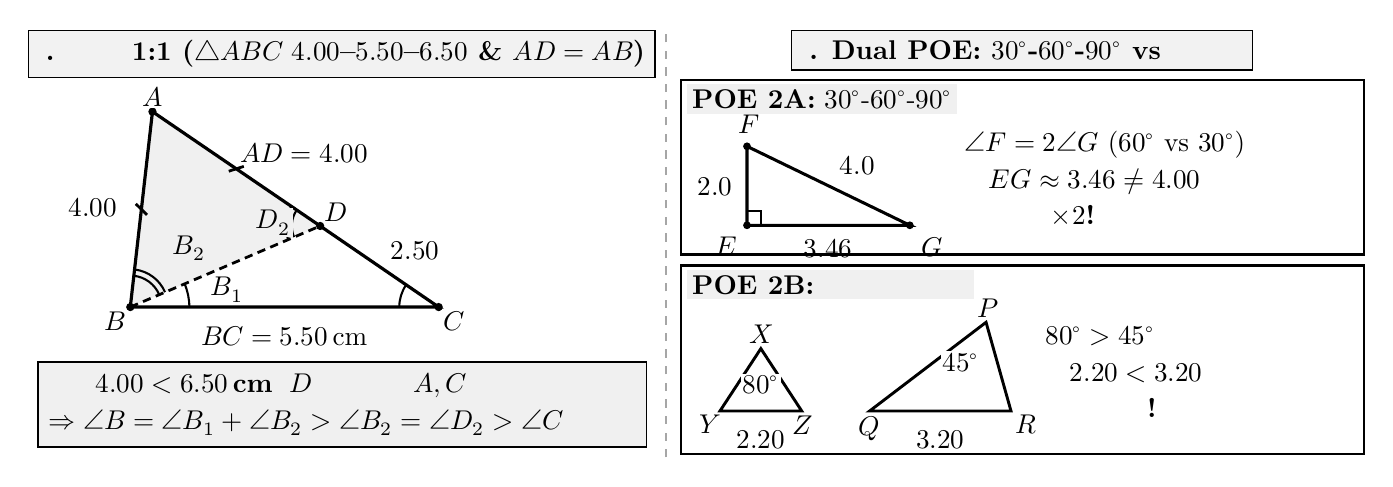
\begin{tikzpicture}[x=0.88cm, y=0.88cm, every node/.style={font=\linespread{1.0}\fontsize{9.8pt}{13.2pt}\selectfont, text=black}]
  \draw[line width=0.6pt, dashed, gray!70] (9.18, 0.05) -- (9.18, 6.24);
  \node[anchor=north, fill=headgray, draw=black, line width=0.5pt, inner sep=3.6pt] at (4.50, 6.22) {\textbf{ក. កាត់បត់ \en{1:1} ($\tri{ABC}$ $4.00\text{--}5.50\text{--}6.50$ \en{\&} $AD=AB$)}};
  \node[anchor=north, fill=headgray, draw=black, line width=0.5pt, inner sep=3.6pt] at (14.32, 6.22) {\textbf{ខ. \en{Dual POE}: $30^\circ\text{-}60^\circ\text{-}90^\circ$ \en{vs} ២ ត្រីកោណ}};

  % Left: Exact 1:1 scaled scalene ABC + slider bar
  \begin{scope}[shift={(1.45, 2.22)}]
    \coordinate (B) at (0.00, 0.00);
    \coordinate (C) at (4.45, 0.00);
    \coordinate (A) at (0.32, 2.82);
    \coordinate (D) at (2.74, 1.17);
    \fill[panelgray] (A) -- (B) -- (D) -- cycle;
    \draw[black, line width=1.15pt, tkslash] (A) -- (B);
    \draw[black, line width=1.15pt, tkslash] (A) -- (D);
    \draw[black, line width=1.15pt] (D) -- (C) -- (B);
    \draw[black, densely dashed, line width=1.0pt] (B) -- (D);
    \pic[draw=black, line width=0.75pt, angle radius=4.0mm]{angle=D--B--A};
    \pic[draw=black, line width=0.75pt, angle radius=4.8mm]{angle=D--B--A};
    \pic[draw=black, line width=0.75pt, angle radius=7.5mm]{angle=C--B--D};
    \pic[draw=black, line width=0.75pt, angle radius=3.6mm]{angle=A--D--B};
    \pic[draw=black, line width=0.75pt, angle radius=4.4mm]{angle=A--D--B};
    \pic[draw=black, line width=0.75pt, angle radius=5.0mm]{angle=A--C--B};
    \fill[black] (A) circle (1.5pt) node[above=1pt, fill=white, inner sep=0.8pt] {\en{$A$}};
    \fill[black] (B) circle (1.5pt) node[below left=1pt, fill=white, inner sep=0.8pt] {\en{$B$}};
    \fill[black] (C) circle (1.5pt) node[below right=1pt, fill=white, inner sep=0.8pt] {\en{$C$}};
    \fill[black] (D) circle (1.5pt) node[above right=1pt, fill=white, inner sep=0.8pt] {\en{$D$}};
    \node[anchor=east] at (-0.05, 1.44) {\en{$4.00$}};
    \node[anchor=south west, fill=white, inner sep=0.8pt] at (1.55, 2.04) {\en{$AD=4.00$}};
    \node[anchor=south west] at (3.62, 0.54) {\en{$2.50$}};
    \node[anchor=north] at (2.22, -0.14) {\en{$BC=5.50\unit{cm}$}};
    \node[fill=panelgray, inner sep=0.8pt] at (0.85, 0.85) {\en{$B_2$}};
    \node[fill=white, inner sep=0.8pt] at (1.40, 0.25) {\en{$B_1$}};
    \node[fill=panelgray, inner sep=0.8pt] at (2.06, 1.22) {\en{$D_2$}};
  \end{scope}
  \node[anchor=north west, draw=black, fill=panelgray, line width=0.65pt, inner sep=4pt, align=left, text width=7.45cm] at (0.10, 1.44) {%
    \textbf{រំកិល $4.00 < 6.50\unit{cm}$៖} $D$ ស្ថិត\textbf{ចន្លោះ} $A, C$\\
    $\Rightarrow \ang{B}=\ang{B_1}+\ang{B_2} > \ang{B_2}=\ang{D_2} > \ang{C}$};

  % Right top: POE 2A (30-60-90)
  \begin{scope}[shift={(9.40, 2.98)}]
    \draw[black, line width=0.85pt] (0, 0) rectangle (9.85, 2.52);
    \node[anchor=north west, fill=panelgray, inner sep=1.8pt] at (0.08, 2.46) {\textbf{\en{POE 2A}:} \en{$30^\circ\text{-}60^\circ\text{-}90^\circ$}};
    \coordinate (E) at (0.95, 0.42);
    \coordinate (G) at (3.30, 0.42);
    \coordinate (F) at (0.95, 1.56);
    \draw[black, line width=1.1pt] (E) -- (G) -- (F) -- cycle;
    \rightanglemark[0.18]{(E)}{(G)}{(F)}
    \fill[black] (E) circle (1.4pt) node[below left=1pt] {\en{$E$}};
    \fill[black] (F) circle (1.4pt) node[above=1pt] {\en{$F$}};
    \fill[black] (G) circle (1.4pt) node[below right=1pt] {\en{$G$}};
    \node[anchor=east] at (0.88, 0.98) {\en{$2.0$}};
    \node[anchor=north] at (2.12, 0.36) {\en{$3.46$}};
    \node[anchor=south west] at (2.15, 1.00) {\en{$4.0$}};
    \node[anchor=west, align=left] at (3.95, 1.10) {\en{$\ang{F}=2\ang{G}$ ($60^\circ$ \en{vs} $30^\circ$)}\\ តែ \en{$EG\approx 3.46\neq 4.00$}\\ \textbf{គ្មានផលធៀប $\times 2$!}};
  \end{scope}

  % Right bottom: POE 2B (Two separate triangles with crisp Z vs Q separation)
  \begin{scope}[shift={(9.40, 0.10)}]
    \draw[black, line width=0.85pt] (0, 0) rectangle (9.85, 2.72);
    \node[anchor=north west, fill=panelgray, inner sep=1.8pt] at (0.08, 2.66) {\textbf{\en{POE 2B}:} ២ ត្រីកោណដាច់ពីគ្នា};
    \coordinate (Y) at (0.56, 0.62);
    \coordinate (Z) at (1.74, 0.62);
    \coordinate (X) at (1.15, 1.52);
    \draw[black, line width=1.05pt] (X) -- (Y) -- (Z) -- cycle;
    \node[above=1pt, fill=white, inner sep=0.8pt] at (X) {\en{$X$}};
    \node[below left=0.8pt, fill=white, inner sep=0.8pt] at (Y) {\en{$Y$}};
    \node[below=0.8pt, fill=white, inner sep=0.8pt] at (Z) {\en{$Z$}};
    \node[anchor=north] at (1.15, 0.48) {\en{$2.20$}};
    \node[fill=white, inner sep=0.6pt] at (1.15, 1.00) {\en{$80^\circ$}};
    \coordinate (Q) at (2.72, 0.62);
    \coordinate (R) at (4.76, 0.62);
    \coordinate (P) at (4.40, 1.90);
    \draw[black, line width=1.05pt] (P) -- (Q) -- (R) -- cycle;
    \node[above=0.8pt, fill=white, inner sep=0.8pt] at (P) {\en{$P$}};
    \node[below=0.8pt, fill=white, inner sep=0.8pt] at (Q) {\en{$Q$}};
    \node[below right=0.8pt, fill=white, inner sep=0.8pt] at (R) {\en{$R$}};
    \node[anchor=north] at (3.74, 0.48) {\en{$3.20$}};
    \node[fill=white, inner sep=0.8pt] at (4.04, 1.32) {\en{$45^\circ$}};
    \node[anchor=west, align=left] at (5.12, 1.18) {\en{$80^\circ > 45^\circ$}\\ តែ \en{$2.20 < 3.20$}\\ \textbf{២ ត្រីកោណដាច់!}};
  \end{scope}
\end{tikzpicture}\par
\vspace{2pt}
{\fontsize{10.5pt}{14pt}\selectfont\textbf{រូបទី ១៖} ការកាត់បត់ \en{1:1} ដោយបន្ទះរំកិល $AD=AB<AC$ និង \en{Dual POE 2A--2B} បដិសេធសមាមាត្រនិងត្រីកោណដាច់ពីគ្នា \en{(Gridos et al., 2019; Winer \& Battista, 2022; De Bock et al., 2003; Biber, 2020)}។}
\end{tcolorbox}

% --- រូបទី ២ ---
\Needspace{6.4cm}
\begin{tcolorbox}[enhanced, sharp corners, colback=white, colframe=black, boxrule=0.8pt, top=4pt, bottom=4pt, left=4pt, right=4pt, before skip=2pt, after skip=4pt]
\centering
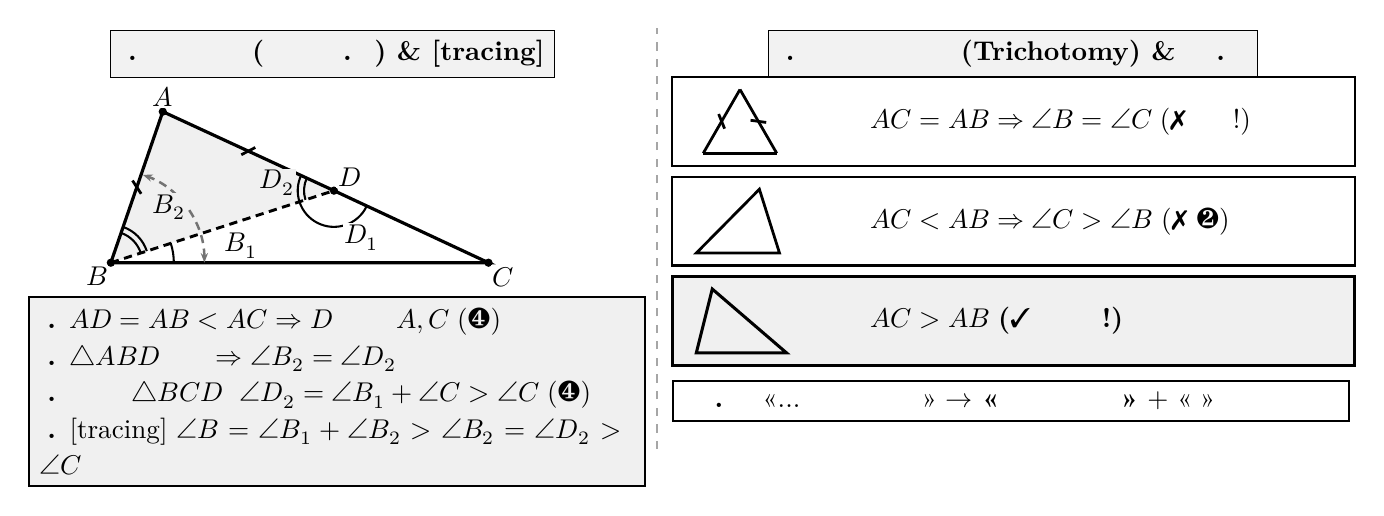
\begin{tikzpicture}[x=0.88cm, y=0.88cm, every node/.style={font=\linespread{1.0}\fontsize{9.8pt}{13.2pt}\selectfont, text=black}]
  \draw[line width=0.6pt, dashed, gray!70] (9.18, 0.05) -- (9.18, 6.12);
  \node[anchor=north, fill=headgray, draw=black, line width=0.5pt, inner sep=3.6pt] at (4.50, 6.10) {\textbf{ក. សម្រាយផ្ទាល់ (ឧទាហរណ៍ ទំ.១៥៨) \& \en{[tracing]}}};
  \node[anchor=north, fill=headgray, draw=black, line width=0.5pt, inner sep=3.6pt] at (14.32, 6.10) {\textbf{ខ. សម្រាយច្រាស ៣ ករណី \en{(Trichotomy)} \& កែទំ.១៥៨}};

  % Left: Direct Proof ABC with tracing
  \begin{scope}[shift={(1.30, 2.74)}]
    \coordinate (B2) at (0.00, 0.00);
    \coordinate (C2) at (5.45, 0.00);
    \coordinate (A2) at (0.75, 2.18);
    \coordinate (D2) at (3.22, 1.04);
    \fill[panelgray] (A2) -- (B2) -- (D2) -- cycle;
    \draw[black, line width=1.15pt, tkslash] (A2) -- (B2);
    \draw[black, line width=1.15pt, tkslash] (A2) -- (D2);
    \draw[black, line width=1.15pt] (D2) -- (C2) -- (B2);
    \draw[black, densely dashed, line width=1.05pt] (B2) -- (D2);
    \draw[bordergray, densely dashed, line width=0.9pt, {Stealth[length=3.5pt]}-{Stealth[length=3.5pt]}]
      ($(B2)+(0:1.35)$) arc (0:70:1.35);
    \pic[draw=black, line width=0.75pt, angle radius=4.0mm]{angle=D2--B2--A2};
    \pic[draw=black, line width=0.75pt, angle radius=4.8mm]{angle=D2--B2--A2};
    \pic[draw=black, line width=0.75pt, angle radius=8.0mm]{angle=C2--B2--D2};
    \pic[draw=black, line width=0.75pt, angle radius=3.8mm]{angle=A2--D2--B2};
    \pic[draw=black, line width=0.75pt, angle radius=4.6mm]{angle=A2--D2--B2};
    \pic[draw=black, line width=0.75pt, angle radius=4.6mm]{angle=B2--D2--C2};
    \fill[black] (A2) circle (1.5pt) node[above=1pt, fill=white, inner sep=0.6pt] {\en{$A$}};
    \fill[black] (B2) circle (1.5pt) node[below left=1pt, fill=white, inner sep=0.6pt] {\en{$B$}};
    \fill[black] (C2) circle (1.5pt) node[below right=1pt, fill=white, inner sep=0.6pt] {\en{$C$}};
    \fill[black] (D2) circle (1.5pt) node[above right=1pt, fill=white, inner sep=0.6pt] {\en{$D$}};
    \node[fill=panelgray, inner sep=0.6pt] at (0.84, 0.80) {\en{$B_2$}};
    \node[fill=white, inner sep=0.6pt] at (1.88, 0.24) {\en{$B_1$}};
    \node[fill=panelgray, inner sep=0.6pt] at (2.40, 1.15) {\en{$D_2$}};
    \node[fill=white, inner sep=0.6pt] at (3.62, 0.36) {\en{$D_1$}};
  \end{scope}
  \node[anchor=north west, draw=black, fill=panelgray, line width=0.7pt, inner sep=4pt, align=left, text width=7.55cm] at (0.10, 2.26) {%
    \textbf{១.} $AD=AB<AC \Rightarrow D$ ចន្លោះ $A,C$ (\cnum{4})\\
    \textbf{២.} $\tri{ABD}$ សមបាទ $\Rightarrow \ang{B_2}=\ang{D_2}$\\
    \textbf{៣.} មុំក្រៅ $\tri{BCD}$៖ $\ang{D_2}=\ang{B_1}+\ang{C}>\ang{C}$ (\cnum{4})\\
    \textbf{៤.} \en{[tracing]} $\ang{B}=\ang{B_1}+\ang{B_2}>\ang{B_2}=\ang{D_2}>\ang{C}$};

  % Right: 3-Case Trichotomy & Erratum #1 Box
  \begin{scope}[shift={(9.40, 4.14)}]
    \draw[black, line width=0.8pt] (0, 0) rectangle (9.85, 1.28);
    \draw[black, line width=1.0pt, tkslash] (0.45, 0.18) -- (0.98, 1.10);
    \draw[black, line width=1.0pt, tkslash] (1.51, 0.18) -- (0.98, 1.10);
    \draw[black, line width=1.0pt] (0.45, 0.18) -- (1.51, 0.18);
    \node[anchor=west, align=left] at (1.78, 0.64) {\textbf{ករណី ១៖} $AC=AB \Rightarrow \ang{B}=\ang{C}$ (\ding{55} ផ្ទុយ!)};
  \end{scope}
  \begin{scope}[shift={(9.40, 2.70)}]
    \draw[black, line width=0.8pt] (0, 0) rectangle (9.85, 1.28);
    \draw[black, line width=1.0pt] (0.35, 0.18) -- (1.55, 0.18) -- (1.26, 1.10) -- cycle;
    \node[anchor=west, align=left] at (1.78, 0.64) {\textbf{ករណី ២៖} $AC<AB \Rightarrow \ang{C}>\ang{B}$ (\ding{55} \cnum{2})};
  \end{scope}
  \begin{scope}[shift={(9.40, 1.26)}]
    \draw[black, line width=1.15pt, fill=panelgray] (0, 0) rectangle (9.85, 1.28);
    \draw[black, line width=1.1pt] (0.35, 0.18) -- (1.65, 0.18) -- (0.58, 1.10) -- cycle;
    \node[anchor=west, align=left] at (1.78, 0.64) {\textbf{ករណី ៣៖} $AC>AB$ \textbf{(\ding{51} សល់តែមួយ!)}};
  \end{scope}
  \node[anchor=north west, draw=black, fill=white, line width=0.75pt, inner sep=4pt, align=left, text width=8.30cm] at (9.40, 1.05) {%
    \textbf{កែទំ.១៥៨៖} «...ក៏មានប៉ុនគ្នាដែរ» $\to$ \textbf{«ក៏មិនប៉ុនគ្នាដែរ»} + «។»};
\end{tikzpicture}\par
\vspace{2pt}
{\fontsize{10.5pt}{14pt}\selectfont\textbf{រូបទី ២៖} សម្រាយផ្ទាល់ទំ.១៥៨ ភ្ជាប់ហេតុផល \en{Betweenness} និងសម្រាយច្រាស ៣ ករណី \en{Trichotomy} កែតម្រូវ \en{Erratum \#1} \en{(Baccaglini-Frank et al., 2013; Winer \& Battista, 2022; Yeo \& Tzeng, 2019; Xu et al., 2026)}។}
\end{tcolorbox}

% --- រូបទី ៣ ---
\Needspace{6.4cm}
\begin{tcolorbox}[enhanced, sharp corners, colback=white, colframe=black, boxrule=0.8pt, top=4pt, bottom=4pt, left=4pt, right=4pt, before skip=2pt, after skip=4pt]
\centering
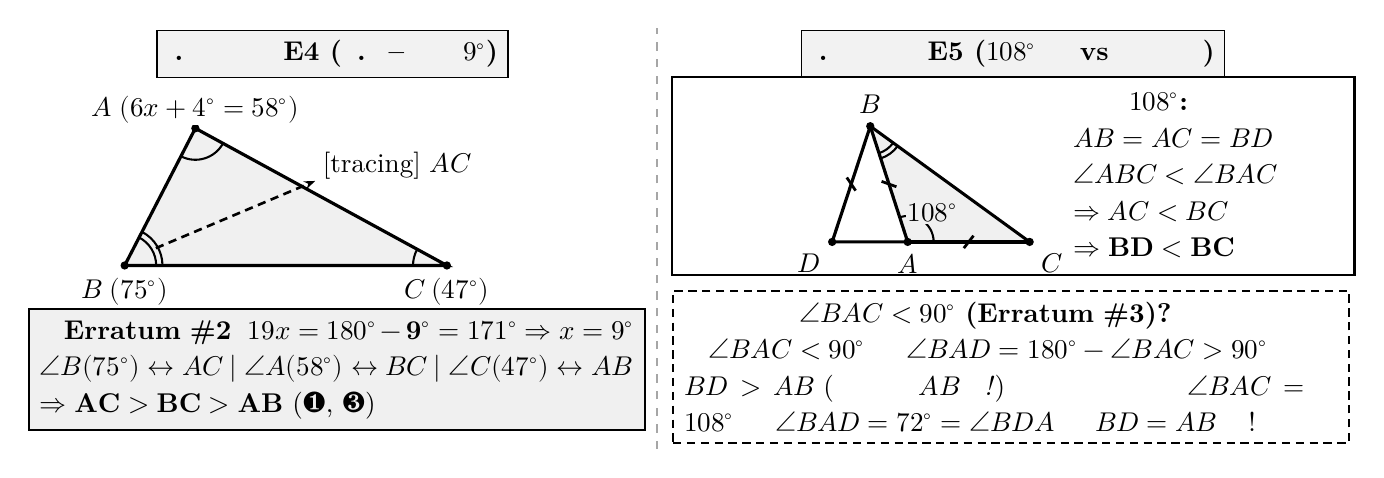
\begin{tikzpicture}[x=0.88cm, y=0.88cm, every node/.style={font=\linespread{1.0}\fontsize{9.8pt}{13.2pt}\selectfont, text=black}]
  \draw[line width=0.6pt, dashed, gray!70] (9.18, 0.05) -- (9.18, 6.12);
  \node[anchor=north, fill=headgray, draw=black, line width=0.5pt, inner sep=3.6pt] at (4.50, 6.10) {\textbf{ក. លំហាត់គំរូ \en{E4} (ទំ.១៥៨\en{--}១៥៩ កែ $9^\circ$)}};
  \node[anchor=north, fill=headgray, draw=black, line width=0.5pt, inner sep=3.6pt] at (14.32, 6.10) {\textbf{ខ. ប្រតិបត្តិ \en{E5} ($108^\circ$ ពិត \en{vs} ស្រួចមិនពិត)}};

  % Left: E4 Model Problem 58-75-47
  \begin{scope}[shift={(1.50, 2.70)}]
    \coordinate (Bm) at (0.00, 0.00);
    \coordinate (Cm) at (4.65, 0.00);
    \coordinate (Am) at (1.02, 1.98);
    \fill[panelgray] (Am) -- (Bm) -- (Cm) -- cycle;
    \draw[black, line width=1.15pt] (Am) -- (Bm) -- (Cm) -- cycle;
    \draw[black, densely dashed, line width=0.95pt, -{Stealth[length=4pt]}] (0.45, 0.25) -- (2.75, 1.22);
    \pic[draw=black, line width=0.75pt, angle radius=4.0mm]{angle=Bm--Am--Cm};
    \pic[draw=black, line width=0.75pt, angle radius=4.0mm]{angle=Cm--Bm--Am};
    \pic[draw=black, line width=0.75pt, angle radius=4.8mm]{angle=Cm--Bm--Am};
    \pic[draw=black, line width=0.75pt, angle radius=4.3mm]{angle=Am--Cm--Bm};
    \fill[black] (Am) circle (1.5pt) node[above=1pt, fill=white, inner sep=0.6pt] {\en{$A\;(6x+4^\circ=58^\circ)$}};
    \fill[black] (Bm) circle (1.5pt) node[below=1pt] {\en{$B\;(75^\circ)$}};
    \fill[black] (Cm) circle (1.5pt) node[below=1pt] {\en{$C\;(47^\circ)$}};
    \node[anchor=south west, fill=white, inner sep=0.8pt] at (2.82, 1.20) {\en{[tracing]} $AC$};
  \end{scope}
  \node[anchor=north west, draw=black, fill=panelgray, line width=0.7pt, inner sep=4pt, align=left, text width=7.55cm] at (0.10, 2.08) {%
    \textbf{កែ \en{Erratum \#2}៖} $19x = 180^\circ - \mathbf{9^\circ} = 171^\circ \Rightarrow x = 9^\circ$\\
    $\ang{B}(75^\circ)\leftrightarrow AC \;\vert\; \ang{A}(58^\circ)\leftrightarrow BC \;\vert\; \ang{C}(47^\circ)\leftrightarrow AB$\\
    $\Rightarrow \mathbf{AC > BC > AB}$ (\cnum{1}, \cnum{3})};

  % Right top: True Obtuse 108 deg Practice figure (with generous top clearance)
  \begin{scope}[shift={(12.80, 3.04)}]
    \draw[black, line width=0.85pt] (-3.40, -0.48) rectangle (6.45, 2.38);
    \coordinate (Ap) at (0.00, 0.00);
    \coordinate (Cp) at (1.76, 0.00);
    \coordinate (Bp) at (-0.54, 1.67);
    \coordinate (Dp) at (-1.09, 0.00);
    \fill[panelgray] (Ap) -- (Bp) -- (Cp) -- cycle;
    \draw[black, line width=1.15pt, tkslash] (Ap) -- (Cp);
    \draw[black, line width=1.15pt, tkslash] (Ap) -- (Bp);
    \draw[black, line width=1.15pt, tkslash] (Bp) -- (Dp);
    \draw[black, line width=1.1pt] (Dp) -- (Ap) (Bp) -- (Cp);
    \pic[draw=black, line width=0.75pt, angle radius=3.3mm]{angle=Cp--Ap--Bp};
    \pic[draw=black, line width=0.75pt, angle radius=3.6mm]{angle=Ap--Bp--Cp};
    \pic[draw=black, line width=0.75pt, angle radius=4.3mm]{angle=Ap--Bp--Cp};
    \fill[black] (Ap) circle (1.5pt) node[below=1pt] {\en{$A$}};
    \fill[black] (Cp) circle (1.5pt) node[below right=1pt] {\en{$C$}};
    \fill[black] (Bp) circle (1.5pt) node[above=1pt] {\en{$B$}};
    \fill[black] (Dp) circle (1.5pt) node[below left=1pt] {\en{$D$}};
    \node[fill=panelgray, inner sep=0.6pt] at (0.36, 0.42) {\en{$108^\circ$}};
    \node[anchor=west, align=left] at (2.25, 0.96) {\textbf{រូបពិត $108^\circ$:}\\ $AB=AC=BD$\\ $\ang{ABC}<\ang{BAC}$\\ $\Rightarrow AC<BC$\\ $\Rightarrow \mathbf{BD<BC}$};
  \end{scope}

  % Right bottom: Impossible Acute BAC warning
  \node[anchor=north west, draw=black, densely dashed, fill=white, line width=0.75pt, inner sep=4pt, align=left, text width=8.30cm] at (9.40, 2.35) {%
    \textbf{ហេតុអ្វីហាមគូស $\ang{BAC}<90^\circ$ (\en{Erratum \#3})?}\\
    បើ $\ang{BAC}<90^\circ$ នោះ $\ang{BAD}=180^\circ-\ang{BAC}>90^\circ$ បង្ខំឱ្យ $BD>AB$ (\textit{មិនអាចស្មើ $AB$ ទេ!}) ដូច្នេះត្រូវគូសមុំទាល $\ang{BAC}=108^\circ$ ទើប $\ang{BAD}=72^\circ=\ang{BDA}$ និង $BD=AB$ ពិត!};
\end{tikzpicture}\par
\vspace{2pt}
{\fontsize{10.5pt}{14pt}\selectfont\textbf{រូបទី ៣៖} លំហាត់គំរូ \en{E4} (ទំ.១៥៨--១៥៩ កែ $9^\circ$ + \en{[tracing]}) និងប្រតិបត្តិ \en{E5} មុំទាល $108^\circ$ ទល់នឹងរូបស្រួចមិនពិត \en{(Ataş-Koçluk \& Tanışlı, 2026; Dietiker et al., 2017; Catman-Aksoy \& Isiksal-Bostan, 2024)}។}
\end{tcolorbox}

% --- រូបទី ៤ ---
\Needspace{7.3cm}
\begin{tcolorbox}[enhanced, sharp corners, colback=white, colframe=black, boxrule=0.8pt, top=4pt, bottom=4pt, left=4pt, right=4pt, before skip=2pt, after skip=4pt]
\centering
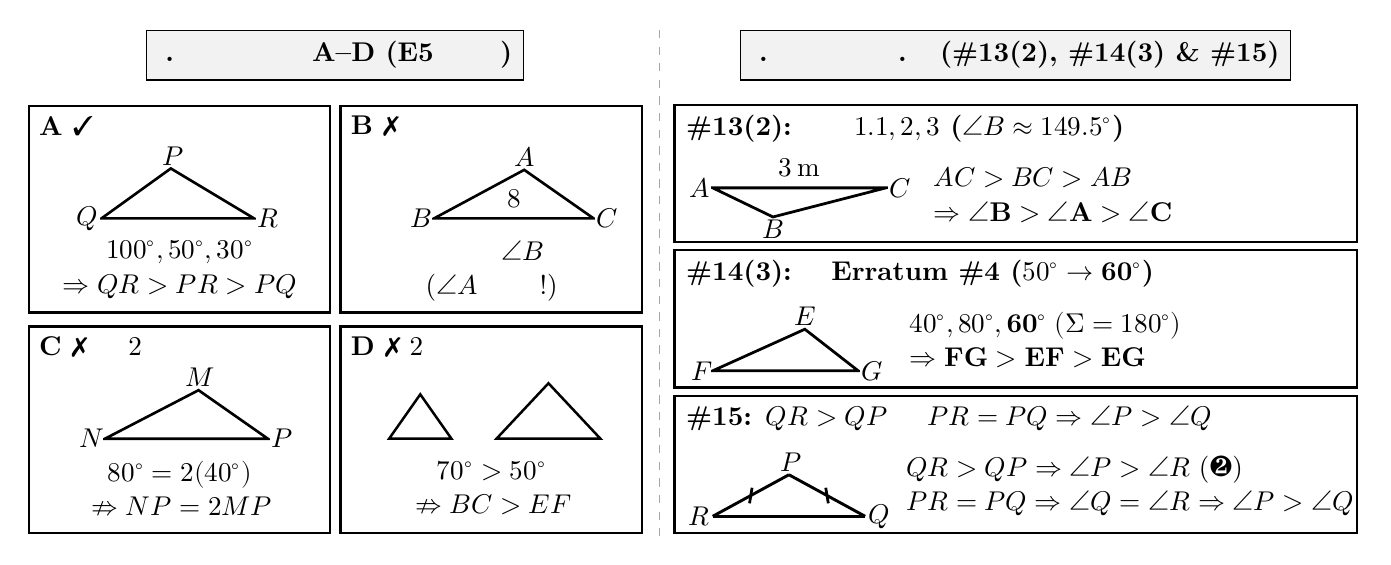
\begin{tikzpicture}[x=0.88cm, y=0.88cm, every node/.style={font=\linespread{1.0}\fontsize{9.8pt}{12.5pt}\selectfont, text=black}]
  \draw[line width=0.6pt, dashed, gray!70] (9.18, 0.05) -- (9.18, 7.38);
  \node[anchor=north, fill=headgray, draw=black, line width=0.5pt, inner sep=4.0pt] at (4.50, 7.36) {\textbf{ក. កាតត្រួតពិនិត្យ \en{A--D} \en{(E5} ទំព័រ ៥\en{)}}};
  \node[anchor=north, fill=headgray, draw=black, line width=0.5pt, inner sep=4.0pt] at (14.32, 7.36) {\textbf{ខ. កិច្ចការផ្ទះ ទំ.១៦៦ \en{(\#13(2), \#14(3) \& \#15)}}};

  % Left 2x2 Cards A-D (each 4.35 x 2.98 with clean margin below header)
  \begin{scope}[shift={(0.08, 3.28)}]
    \draw[black, line width=0.8pt] (0,0) rectangle (4.35, 2.98);
    \node[anchor=north west, inner sep=2pt] at (0.06, 2.92) {\textbf{\en{A} \ding{51}}};
    \coordinate (pA) at (2.05, 2.08); \coordinate (qA) at (1.05, 1.36); \coordinate (rA) at (3.25, 1.36);
    \draw[black, line width=0.95pt] (pA)--(qA)--(rA)--cycle;
    \node[above=0.5pt, fill=white, inner sep=0.5pt] at (pA) {\en{$P$}}; \node[left=0.5pt, fill=white, inner sep=0.5pt] at (qA) {\en{$Q$}}; \node[right=0.5pt, fill=white, inner sep=0.5pt] at (rA) {\en{$R$}};
    \node[anchor=north, align=center] at (2.18, 1.18) {\en{$100^\circ, 50^\circ, 30^\circ$}\\ \en{$\Rightarrow QR>PR>PQ$}};
  \end{scope}
  \begin{scope}[shift={(4.58, 3.28)}]
    \draw[black, line width=0.8pt] (0,0) rectangle (4.35, 2.98);
    \node[anchor=north west, inner sep=2pt] at (0.06, 2.92) {\textbf{\en{B} \ding{55}} កំពូលឈម};
    \coordinate (aB) at (2.65, 2.06); \coordinate (bB) at (1.35, 1.36); \coordinate (cB) at (3.65, 1.36);
    \draw[black, line width=0.95pt] (aB)--(bB)--(cB)--cycle;
    \node[above=0.5pt, fill=white, inner sep=0.5pt] at (aB) {\en{$A$}}; \node[left=0.5pt, fill=white, inner sep=0.5pt] at (bB) {\en{$B$}}; \node[right=0.5pt, fill=white, inner sep=0.5pt] at (cB) {\en{$C$}};
    \node[anchor=south] at (2.50, 1.36) {\en{$8$}};
    \node[anchor=north, align=center] at (2.18, 1.18) {អន្ទាក់ $\ang{B}$\\ ($\ang{A}$ ធំបំផុត!)};
  \end{scope}
  \begin{scope}[shift={(0.08, 0.10)}]
    \draw[black, line width=0.8pt] (0,0) rectangle (4.35, 2.98);
    \node[anchor=north west, inner sep=2pt] at (0.06, 2.92) {\textbf{\en{C} \ding{55}} គុណ \en{2}};
    \coordinate (mC) at (2.45, 2.06); \coordinate (nC) at (1.10, 1.36); \coordinate (pC) at (3.45, 1.36);
    \draw[black, line width=0.95pt] (mC)--(nC)--(pC)--cycle;
    \node[above=0.5pt, fill=white, inner sep=0.5pt] at (mC) {\en{$M$}}; \node[left=0.5pt, fill=white, inner sep=0.5pt] at (nC) {\en{$N$}}; \node[right=0.5pt, fill=white, inner sep=0.5pt] at (pC) {\en{$P$}};
    \node[anchor=north, align=center] at (2.18, 1.18) {\en{$80^\circ=2(40^\circ)$}\\ \en{$\not\Rightarrow NP=2MP$}};
  \end{scope}
  \begin{scope}[shift={(4.58, 0.10)}]
    \draw[black, line width=0.8pt] (0,0) rectangle (4.35, 2.98);
    \node[anchor=north west, inner sep=2pt] at (0.06, 2.92) {\textbf{\en{D} \ding{55}} \en{2} ត្រីកោណ};
    \draw[black, line width=0.9pt] (0.70, 1.36) -- (1.60, 1.36) -- (1.15, 2.00) -- cycle;
    \draw[black, line width=0.9pt] (2.25, 1.36) -- (3.75, 1.36) -- (3.00, 2.16) -- cycle;
    \node[anchor=north, align=center] at (2.18, 1.18) {\en{$70^\circ>50^\circ$}\\ \en{$\not\Rightarrow BC>EF$}};
  \end{scope}

  % Right: HW #13(2), #14(3) fix, #15 (3 stacked boxes height 1.98 each)
  \begin{scope}[shift={(9.40, 4.30)}]
    \draw[black, line width=0.8pt] (0,0) rectangle (9.85, 1.98);
    \node[anchor=north west, inner sep=2pt] at (0.08, 1.92) {\textbf{\en{\#13(2):} ជឿលេខ $1.1, 2, 3$ ($\ang{B}\approx 149.5^\circ$)}};
    \coordinate (a13) at (0.55, 0.78); \coordinate (c13) at (3.05, 0.78); \coordinate (b13) at (1.42, 0.36);
    \draw[black, line width=1.0pt] (a13)--(b13)--(c13)--cycle;
    \node[left=0.5pt, fill=white, inner sep=0.5pt] at (a13) {\en{$A$}}; \node[right=0.5pt, fill=white, inner sep=0.5pt] at (c13) {\en{$C$}}; \node[below=0.5pt, fill=white, inner sep=0.5pt] at (b13) {\en{$B$}};
    \node[anchor=south] at (1.80, 0.79) {\en{$3\unit{m}$}};
    \node[anchor=west, align=left] at (3.60, 0.68) {\en{$AC>BC>AB$}\\ $\Rightarrow \mathbf{\ang{B}>\ang{A}>\ang{C}}$};
  \end{scope}
  \begin{scope}[shift={(9.40, 2.20)}]
    \draw[black, line width=0.8pt] (0,0) rectangle (9.85, 1.98);
    \node[anchor=north west, inner sep=2pt] at (0.08, 1.92) {\textbf{\en{\#14(3):} កែ \en{Erratum \#4} ($50^\circ \to \mathbf{60^\circ}$)}};
    \coordinate (f14) at (0.55, 0.24); \coordinate (g14) at (2.65, 0.24); \coordinate (e14) at (1.88, 0.84);
    \draw[black, line width=1.0pt] (f14)--(e14)--(g14)--cycle;
    \node[left=0.5pt, fill=white, inner sep=0.5pt] at (f14) {\en{$F$}}; \node[above=0.5pt, fill=white, inner sep=0.5pt] at (e14) {\en{$E$}}; \node[right=0.5pt, fill=white, inner sep=0.5pt] at (g14) {\en{$G$}};
    \node[anchor=west, align=left] at (3.25, 0.68) {\en{$40^\circ, 80^\circ, \mathbf{60^\circ}\;(\Sigma=180^\circ)$}\\ $\Rightarrow \mathbf{FG>EF>EG}$};
  \end{scope}
  \begin{scope}[shift={(9.40, 0.10)}]
    \draw[black, line width=0.8pt] (0,0) rectangle (9.85, 1.98);
    \node[anchor=north west, inner sep=2pt] at (0.08, 1.92) {\textbf{\en{\#15:} $QR>QP$ និង $PR=PQ \Rightarrow \ang{P}>\ang{Q}$}};
    \coordinate (r15) at (0.55, 0.24); \coordinate (q15) at (2.75, 0.24); \coordinate (p15) at (1.65, 0.84);
    \draw[black, line width=1.05pt, tkslash] (p15)--(r15);
    \draw[black, line width=1.05pt, tkslashR] (p15)--(q15);
    \draw[black, line width=1.05pt] (r15)--(q15);
    \node[above=0.5pt, fill=white, inner sep=0.5pt] at (p15) {\en{$P$}}; \node[left=0.5pt, fill=white, inner sep=0.5pt] at (r15) {\en{$R$}}; \node[right=0.5pt, fill=white, inner sep=0.5pt] at (q15) {\en{$Q$}};
    \node[anchor=west, align=left] at (3.20, 0.68) {\en{$QR>QP \Rightarrow \ang{P}>\ang{R}$ (\cnum{2})}\\ \en{$PR=PQ \Rightarrow \ang{Q}=\ang{R} \Rightarrow \ang{P}>\ang{Q}$}};
  \end{scope}
\end{tikzpicture}\par
\vspace{2pt}
{\fontsize{10.5pt}{14pt}\selectfont\textbf{រូបទី ៤៖} កាតវិនិច្ឆ័យ \en{A--D} (ទំព័រ ៥) និងគំនូសកិច្ចការផ្ទះទំព័រ ១៦៦ (\en{\#13(2), \#14(3)} កែ $60^\circ$ និង \en{\#15}) \en{(Dietiker et al., 2017; De Bock et al., 2003; Scristia et al., 2022)}។}
\end{tcolorbox}

% ============================================================================
% ផ្នែកទី ៦៖ មគ្គុទ្ទេសក៍រៀបចំ និងប្រើប្រាស់សម្ភារៈបោះពុម្ព (Pages 1--6) & ចម្លើយពេញលេញ
% ============================================================================
\secbanner{ផ្នែកទី ៦៖ មគ្គុទ្ទេសក៍រៀបចំ និងប្រើប្រាស់សម្ភារៈបោះពុម្ព \enbf{(Pages 1--6)}}{Section 6: Printing Calibration (Actual Size 100\%), Cut-Out Preparation \& Complete Master Answer Keys}

\subsec{៦\enbf{.}១ ស្តង់ដារបោះពុម្ព \enbf{Actual Size 100\%} និងលំដាប់ចែកសន្លឹកកិច្ចការ}

\begin{enumerate}[leftmargin=0.65cm, itemsep=1.2pt]
  \item \textbf{ការកំណត់បោះពុម្ព \en{1:1} ដាច់ខាត (ទំព័រ ១)៖} បោះពុម្ពឯកសារ \en{Printable\_Materials\_INEQ1.pdf} ដោយជ្រើស \textbf{\en{Scale: Actual Size 100\%}} (\textit{ហាមប្រើ} \en{Fit to Page / Shrink to Fit}) ហើយវាស់ផ្ទៀង\textbf{បន្ទះក្រិត \en{5.00 cm}} (\en{141.73 pt}) នៅខាងស្ដាំផ្នែកខាងលើទំព័រ ១ ដើម្បីធានាថា $\tri{ABC}$ ($AB=4.00, BC=5.50, AC=6.50\unit{cm}$), បន្ទះរំកិល $AD=AB=4.00\unit{cm}$, \en{POE 2A} ($\tri{EFG}$ $30^\circ\text{-}60^\circ\text{-}90^\circ$) និង \en{POE 2B} ($\tri{XYZ}$ $2.20\unit{cm}$ \en{vs} $\tri{PQR}$ $3.20\unit{cm}$) មានខ្នាត \en{1:1} ពិតប្រាកដ។
  \item \textbf{ទម្រង់សន្សំក្រដាស ស-ខ្មៅ (ទំព័រ ២--៦)៖} ទំព័រ ២ (កាត \en{E4} លំហាត់គំរូ) និងទំព័រ ៣ (សន្លឹក \en{E5} ប្រតិបត្តិ ៣ តួនាទី) ជាទម្រង់ \en{2-up} (២ ប័ណ្ណ/សន្លឹកក្នុង ១ ទំព័រ \en{A4}), ទំព័រ ៤ (ផ្ទាំងសំអាងគោល ៣.១ និងធនាគារ \cnum{1}--\cnum{5}) គួរបោះពុម្ពលើក្រដាសរឹង \en{180 gsm} បិទលើក្ដារខៀន, ទំព័រ ៥ ជាកាត \en{A--D} \en{4-up} + ចម្លើយគ្រូ + សំបុត្រចេញ ៣ សំណួរ, និងទំព័រ ៦ ជាប័ណ្ណកិច្ចការផ្ទះ \en{4-up}។
  \item \textbf{ឧបករណ៍តុក្រុម ៣ នាក់ និងកាលវិភាគចែកសន្លឹក៖} កន្ត្រៃ ១, បន្ទាត់ក្រិត \en{cm/mm} ១, រ៉ាព័រទ័រ ១, និងខ្មៅដៃ \en{[tracing]} ក្នុងមួយក្រុម។ ចែកទំព័រ ១ ផ្កាប់លើតុនៅនាទី ០០', ទំព័រ ២ នៅនាទី ២៨', ទំព័រ ៣ នៅនាទី ៣៨', បង្ហាញទំព័រ ៥ នៅនាទី ៤៤.៥', និងចែកទំព័រ ៦ នៅនាទី ៤៨'។
\end{enumerate}

\Needspace{5.8cm}
\subsec{៦\enbf{.}២ ចម្លើយគំរូពេញលេញសម្រាប់គ្រប់សន្លឹកកិច្ចការ និងលំហាត់ \enbf{(Pages 1--6 \& HW)}}

\begingroup
\linespread{1.01}\fontsize{10.2pt}{14.2pt}\selectfont
\renewcommand{\arraystretch}{1.04}
\begin{longtable}{|L{2.95cm}|L{13.90cm}|}
\hline
\rowcolor{headgray}
\multicolumn{1}{|C{2.95cm}|}{\tblhead{សន្លឹក \enbf{/} លំហាត់}} &
\multicolumn{1}{C{13.90cm}|}{\tblhead{ចម្លើយគំរូផ្លូវការ និងពិន្ទុត្រួតពិនិត្យ \enbf{(Master Key)}}} \\
\hline
\endfirsthead
\hline
\rowcolor{headgray}
\multicolumn{1}{|C{2.95cm}|}{\tblhead{សន្លឹក \enbf{/} លំហាត់}} &
\multicolumn{1}{C{13.90cm}|}{\tblhead{ចម្លើយគំរូផ្លូវការ និងពិន្ទុត្រួតពិនិត្យ \enbf{(Master Key)}}} \\
\hline
\endhead
\hline
\endfoot
\hline
\endlastfoot
\textbf{ទំព័រ ១ (\en{E2})} \newline ស.១ កាត់បត់ \en{1:1} \newline ($\tri{ABC}$ \& រំកិល) &
\textbf{សកម្មភាព ១ ($\tri{ABC}$ $AB=4.00\unit{cm}, BC=5.50\unit{cm}, AC=6.50\unit{cm}$ + បន្ទះរំកិល $AD=AB=4.00\unit{cm}$):} \newline
$\bullet$ ដោយ $AD=AB=4.00\unit{cm} < AC=6.50\unit{cm}$ ចំណុច $D$ ស្ថិតនៅ\textbf{ចន្លោះ} $A$ និង $C$ (សល់ $DC=2.50\unit{cm}$)។ \newline
$\bullet$ $AD=AB=4.00\unit{cm} \Rightarrow \tri{ABD}$ \textbf{សមបាទ}កំពូល $A \Rightarrow \ang{B_2} = \mathbf{\ang{D_2}}$ ($61.3^\circ$)។ \newline
$\bullet$ $\ang{D_2}$ ជា\textbf{មុំក្រៅ}នៃ $\tri{BCD} \Rightarrow \ang{D_2}=\ang{B_1}+\ang{C} \Rightarrow \ang{D_2} > \mathbf{\ang{C}}$ ($37.8^\circ$)។ \newline
$\bullet$ បន្ថែមមុំ៖ $\ang{B}=\ang{B_1}+\ang{B_2} > \ang{B_2}=\ang{D_2} > \ang{C} \Rightarrow \ang{B} \;\mathbf{>}\; \ang{C}$ ($84.8^\circ > 37.8^\circ$)។ \\
\hline
\textbf{ទំព័រ ១ (\en{E2})} \newline \en{Dual POE 2A--2B} &
\textbf{\en{POE 2A} ($\tri{EFG}$ $30^\circ\text{--}60^\circ\text{--}90^\circ$):} $EF=\mathbf{2.00\unit{cm}},\; EG\approx \mathbf{3.46\unit{cm}},\; FG=\mathbf{4.00\unit{cm}}$; លំដាប់៖ $FG > EG > EF$។ ពិនិត្យផលធៀប៖ $\ang{F}=2\ang{G}$ តែ $EG\approx 3.46\neq 2(2.00)=4.00\unit{cm}$ (\textbf{មិនស្មើ}) និង $\ang{E}=3\ang{G}$ តែ $FG=4.00\neq 3(2.00)=6.00\unit{cm}$ (\textbf{មិនស្មើ}) — រក្សាតែលំដាប់ មិនរក្សាផលធៀបគុណ! \newline
\textbf{\en{POE 2B} ($\tri{XYZ}$ \en{vs} $\tri{PQR}$):} $YZ=\mathbf{2.20\unit{cm}}$ (ឈម $80^\circ$) និង $QR=\mathbf{3.20\unit{cm}}$ (ឈម $45^\circ$) $\Rightarrow \mathbf{YZ < QR}$ ទោះ $80^\circ > 45^\circ$ (ព្រោះ ២ ត្រីកោណដាច់ពីគ្នា គ្មានស្ពានស្មើភ្ជាប់!)។ \\
\hline
\textbf{ទំព័រ ២ (\en{E4})} \newline លំហាត់គំរូ \newline (ទំ.១៥៨--១៥៩ កែ) &
\textbf{ជំហាន ១ (កែ \en{Erratum \#2} $9^\circ$):} $\ang{A}+\ang{B}+\ang{C}=180^\circ$ (\cnum{5}) $\Rightarrow (6x+4^\circ)+(7x+12^\circ)+(6x-7^\circ)=180^\circ \Rightarrow 19x+9^\circ=180^\circ \Rightarrow 19x=180^\circ-\mathbf{9^\circ}=171^\circ \Rightarrow \mathbf{x=9^\circ}$។ \newline
$\Rightarrow \ang{A}=6(9^\circ)+4^\circ=\mathbf{58^\circ}$, $\ang{B}=7(9^\circ)+12^\circ=\mathbf{75^\circ}$, $\ang{C}=6(9^\circ)-7^\circ=\mathbf{47^\circ}$ ($\Sigma=180^\circ$ \ding{51})។ \newline
\textbf{ជំហាន ២ (តារាង ៣ ជួរ \en{[tracing]} \& \cnum{1}, \cnum{3}):} (១) ធំជាងគេ $\ang{B}=\mathbf{75^\circ}$ $\vert$ អត់ $B \to A,C$ $\vert$ ឈម $\mathbf{AC}$; (២) កណ្ដាល $\ang{A}=\mathbf{58^\circ}$ $\vert$ អត់ $A \to B,C$ $\vert$ ឈម $\mathbf{BC}$; (៣) តូចជាងគេ $\ang{C}=\mathbf{47^\circ}$ $\vert$ អត់ $C \to A,B$ $\vert$ ឈម $\mathbf{AB}$ $\Rightarrow \mathbf{AC > BC > AB}$ (\cnum{3})។ \newline
\textbf{\en{EIA 30s}:} ១) $\ang{B}=75^\circ$ ឈម $AC$ ព្រោះ $B$ ជាកំពូល $\Rightarrow$ អក្សរទី ៣ បាត់គឺ $A, C$។ ២) មិនយក $75^\circ/47^\circ = AC/AB$ ព្រោះ $x$ ជាអញ្ញាត និងមុំមិនសមាមាត្រជ្រុងទេ! \\
\hline
\textbf{ទំព័រ ៣ (\en{E5})} \newline ប្រតិបត្តិ ៣ តួនាទី \newline (ទំ.១៥៩ កែ $108^\circ$) &
\textbf{តួនាទី ១ (\en{[tracing] \& Pause-Ask}):} អូសជុំវិញ $\tri{ABC}$ និងគូស \tickslash{} លើ $AB=AC=BD$។ ហេតុអ្វីមិនមើលតែ $\tri{ABD}$? ព្រោះ $\tri{ABD}$ ខ្វះជ្រុង $BC$! \newline
\textbf{តួនាទី ២ (ស្ពានអង្កត់ស្មើ):} ជំហាន ១ ក្នុង $\tri{ABC}$: $\ang{ABC}<\ang{BAC}$; $\ang{ABC}$ ឈម \textbf{$AC$} (\cnum{1}), $\ang{BAC}$ ឈម \textbf{$BC$} (\cnum{1}) $\Rightarrow \mathbf{AC < BC}$ (\cnum{3})។ ជំហាន ២: ដោយ $AB=AC=BD$ (\cnum{5}) ជំនួស $AC$ ដោយ \textbf{$BD$} $\Rightarrow \mathbf{BD < BC}$ (ពិត!)។ \newline
\textbf{តួនាទី ៣ (\en{Pause-Review \& E1}):} ១) $\ang{BAC}=108^\circ > 90^\circ$ ព្រោះបើស្រួច នោះ $\ang{BAD}>90^\circ \Rightarrow BD>AB$ មិនអាចស្មើគ្នាបានទេ ($\ang{BAD}=72^\circ=\ang{BDA}$ ទើបពិត!)។ ២) សំអាង \cnum{1}, \cnum{3}, \cnum{5} គ្រប់។ \textbf{បិទ \en{E1}:} ដងស្ទូច $4\unit{m}, 7\unit{m}$: មុំហ៊ីងបើកធំ ខ្សែកាបឈមវែងតាមលំដាប់ (\cnum{2}, \cnum{3}) តែមុំគុណ ២ មិននាំឱ្យខ្សែកាបគុណ ២ ឡើយ! \\
\hline
\textbf{ទំព័រ ៤} \newline ផ្ទាំងសំអាង ៣.១ \newline (\cnum{1}--\cnum{5} \en{\& 3 Cases}) &
\textbf{ឧទាហរណ៍ផ្ទាល់ (ទំ.១៥៨)៖} ១) $AD=AB<AC\Rightarrow D$ ចន្លោះ $A,C$ (\cnum{4}); ២) $\tri{ABD}$ សមបាទ $\Rightarrow\ang{B_2}=\ang{D_2}$; ៣) មុំក្រៅ $\tri{BCD}\Rightarrow\ang{D_2}=\ang{B_1}+\ang{C}>\ang{C}$ (\cnum{4}); ៤) $\ang{B}>\ang{C}$។ \textbf{ប្រអប់ទ្រឹស្ដីបទ (កែ \en{Erratum \#1}):} ផ្ទាល់ចប់ដោយ «។»; ច្រាសកែជា «\textbf{ក៏មិនប៉ុនគ្នាដែរ}» + ៣ ករណី \en{Trichotomy} ($AC=AB$ \ding{55}, $AC<AB$ \ding{55}, $AC>AB$ \ding{51})។ \newline
\textbf{ធនាគារ \cnum{1}--\cnum{5}៖} \cnum{1} ស្ពានមុំឈម–ជ្រុងឈម (ក្បួនអក្សរទី ៣ បាត់) $\vert$ \cnum{2} ទ្រឹស្ដីបទផ្ទាល់ ៣.១ ($AC>AB\Rightarrow\ang{B}>\ang{C}$) $\vert$ \cnum{3} ទ្រឹស្ដីបទច្រាស ៣.១ ($\ang{B}>\ang{C}\Rightarrow AC>AB$) $\vert$ \cnum{4} សំណង់ $D$ ($AD=AB<AC$) និងមុំក្រៅ $\ang{D_2}>\ang{C}$ $\vert$ \cnum{5} ផលបូក $180^\circ$ / ៣ ករណី / ស្ពានស្មើ ($BD=AC$)។ \\
\hline
\textbf{ទំព័រ ៥} \newline កាត \en{A--D} \newline \& សំបុត្រចេញ &
\textbf{កាត \en{A} (\ding{51}):} $\ang{P}=100^\circ>\ang{Q}=50^\circ>\ang{R}=30^\circ$ ក្នុង $\tri{PQR}$ តែមួយ $\Rightarrow \mathbf{QR>PR>PQ}$ (\cnum{1}, \cnum{3})។ \newline
\textbf{កាត \en{B} (\ding{55}):} អន្ទាក់កំពូលឈម! $BC=8$ បាត់អក្សរ $A \Rightarrow \mathbf{\ang{A}}$ ទើបជាមុំធំជាងគេ (មិនមែន $\ang{B}$ ទេ)។ \newline
\textbf{កាត \en{C} (\ding{55}):} អន្ទាក់ផលធៀប! $\ang{M}=80^\circ=2\ang{N}$ មិននាំឱ្យ $NP=2MP$ ទេ (ពិតតែ $NP>MN>MP$)។ \newline
\textbf{កាត \en{D} (\ding{55}):} ២ ត្រីកោណដាច់ពីគ្នា! គ្មានស្ពានស្មើភ្ជាប់ $\tri{ABC}$ និង $\tri{DEF}$ ទេ ($BC < EF$)។ \newline
\textbf{សំបុត្រចេញ ៣ សំណួរ:} \textbf{១)} $\tri{KLM}$ ($\ang{K}=52^\circ, \ang{L}=71^\circ$) $\Rightarrow \ang{M}=\mathbf{57^\circ}$, ជ្រុង៖ $\mathbf{KM > KL > LM}$។ \textbf{២)} \textbf{ទេ} — ទ្រឹស្ដីរក្សាលំដាប់ មិនរក្សាផលធៀបទេ។ \textbf{៣)} \cnum{2} (ផ្ទាល់ $\Rightarrow\ang{C}>\ang{B}$ ផ្ទុយ!)។ \\
\hline
\textbf{ទំព័រ ៦ (ផ្ទះ)} \newline ទំ.១៦៦ \newline \en{\#13, \#14, \#15} &
\textbf{លំហាត់ \en{\#13} (មុំពីធំទៅតូច):} \textbf{(1)} $\tri{DEF}$ ($3, 4, 5\unit{cm}$): $EF>DF>DE \Rightarrow \mathbf{\ang{D}>\ang{E}>\ang{F}}$ (\cnum{1}, \cnum{2}); \textbf{(2)} $\tri{ABC}$ ($1.1, 2, 3\unit{m}$): $AC>BC>AB \Rightarrow \mathbf{\ang{B}>\ang{A}>\ang{C}}$ (\textit{ជឿលេខ ទោះរូបគូរស្រួច ខណៈមុំពិត $\ang{B}\approx 149.5^\circ$!}); \textbf{(3)} $\tri{KLM}$ ($2.3, 5.8, 7.6\unit{km}$): $KM>LM>KL \Rightarrow \mathbf{\ang{L}>\ang{K}>\ang{M}}$។ \newline
\textbf{លំហាត់ \en{\#14} (ជ្រុងពីវែងទៅខ្លី):} \textbf{(1)} $\tri{ABC}$ ($90^\circ, 60^\circ, 30^\circ$) $\Rightarrow \mathbf{BC>AC>AB}$ (\cnum{1}, \cnum{3}); \textbf{(2)} $\tri{STR}$ ($24^\circ, 137^\circ, 19^\circ$) $\Rightarrow \mathbf{SR>TR>ST}$; \textbf{(3)} $\tri{FEG}$ \textbf{កែ \en{Erratum \#4}}: សៀវភៅខុស $40^\circ, 80^\circ, 50^\circ$ ($170^\circ$) $\to$ កែឯកភាព \textbf{$40^\circ, 80^\circ, 60^\circ$} ($\Sigma=180^\circ$) $\Rightarrow \mathbf{FG>EF>EG}$ (\cnum{1}, \cnum{3})។ \newline
\textbf{លំហាត់ \en{\#15}:} ក្នុង $\tri{PQR}$, ដោយ $QR>QP \Rightarrow \ang{P}>\ang{R}$ (\cnum{1}, \cnum{2}); ដោយ $PR=PQ \Rightarrow \tri{PQR}$ សមបាទកំពូល $P \Rightarrow \ang{Q}=\ang{R}$; ជំនួស (\cnum{5}) បាន $\mathbf{\ang{P}>\ang{Q}}$ (ពិត!)។ \\
\hline
\end{longtable}
\endgroup

% ============================================================================
% ផ្នែកទី ៧៖ បញ្ជីឯកសារយោង (References --- APA 7th Edition) & ហត្ថលេខា
% ============================================================================
\vspace{2pt}
\secbanner{ផ្នែកទី ៧៖ បញ្ជីឯកសារយោង \enbf{(References --- APA 7th Edition)}}{Section 7: Verified Open-Access Reference List (100\% 1-to-1 Match with PDFs 01--14)}

{\TimesEn\linespread{1.0}\selectfont\fontsize{10.8pt}{16.2pt}\selectfont
\setlength{\parskip}{3.5pt}
\everypar={\hangindent=0.85cm \hangafter=1}

Altıparmak, K., \& Gürcan, G. (2021). Examination of 4th grade students' definitions for square, rectangle and triangle geometric shapes. \textit{Education Quarterly Reviews}, \textit{4}(3), 304--321. \url{https://doi.org/10.31014/aior.1993.04.03.340}

Ataş-Koçluk, Y., \& Tanışlı, D. (2026). Algebraic thinking in the context of geometry and measurement: Eighth-grade students' reasoning processes. \textit{Journal of Pedagogical Research}, \textit{10}(5), 1--29. \url{https://doi.org/10.33902/JPR.202641940}

Baccaglini-Frank, A., Antonini, S., Leung, A., \& Mariotti, M. A. (2013). Reasoning by contradiction in dynamic geometry. \textit{PNA}, \textit{7}(2), 63--73. \url{https://doi.org/10.30827/pna.v7i2.6129}

Biber, A. Ç. (2020). Students' difficulties in similar triangle questions. \textit{Cypriot Journal of Educational Sciences}, \textit{15}(5), 1146--1159. \url{https://doi.org/10.18844/cjes.v15i5.5161}

Biber, Ç., Tuna, A., \& Korkmaz, S. (2013). The mistakes and the misconceptions of the eighth grade students on the subject of angles. \textit{European Journal of Science and Mathematics Education}, \textit{1}(2), 50--59. \url{https://doi.org/10.30935/scimath/9387}

Catman-Aksoy, E., \& Isiksal-Bostan, M. (2024). Fostering students' definitions and images in parallelism and perpendicularity: A paper folding activity. \textit{European Journal of Science and Mathematics Education}, \textit{12}(2), 236--257. \url{https://doi.org/10.30935/scimath/14360}

De Bock, D., Verschaffel, L., Janssens, D., Van Dooren, W., \& Claes, K. (2003). Do realistic contexts and graphical representations always have a beneficial impact on students' performance? Negative evidence from a study on modelling non-linear geometry problems. \textit{Learning and Instruction}, \textit{13}(4), 441--463. \url{https://doi.org/10.1016/S0959-4752(02)00040-3}

Dietiker, L., Brakoniecki, A., \& Riling, M. (2017). The changing expectations for the reading of geometric diagrams. In E. Galindo \& J. Newton (Eds.), \textit{Proceedings of the 39th Annual Meeting of the North American Chapter of the International Group for the Psychology of Mathematics Education} (pp. 136--143). Hoosier Association of Mathematics Teacher Educators. (ERIC Document No. ED581303). \url{https://files.eric.ed.gov/fulltext/ED581303.pdf}

Gridos, P., Gagatsis, A., Elia, I., \& Deliyianni, E. (2019). Mathematical creativity and geometry: The influence of geometrical figure apprehension on the production of multiple solutions. In \textit{Proceedings of the Eleventh Congress of the European Society for Research in Mathematics Education (CERME11)}, Utrecht University, Utrecht, Netherlands. HAL Open Science. \url{https://hal.science/hal-02402180/document}

Miyazaki, M., Nagata, J., Chino, K., Sasa, H., Fujita, T., Komatsu, K., \& Shimizu, S. (2019). Curriculum development for explorative proving in lower secondary school geometry: Focusing on the levels of planning and constructing a proof. \textit{Frontiers in Education}, \textit{4}, Article 31. \url{https://doi.org/10.3389/feduc.2019.00031}

Scristia, Aisyah, S., Meryansumayeka, Safitri, E. R., \& Kurniawan, H. (2022). Students' errors in solving reasoning-based congruence proof problems. \textit{AKSIOMA: Jurnal Program Studi Pendidikan Matematika}, \textit{11}(4), 3160--3167. \url{https://doi.org/10.24127/ajpm.v11i4.5825}

Winer, M. L., \& Battista, M. T. (2022). Investigating students' proof reasoning: Analyzing students' oral proof explanations and their written proofs in high school geometry. \textit{International Electronic Journal of Mathematics Education}, \textit{17}(2), Article em0677. \url{https://doi.org/10.29333/iejme/11713}

Xu, Z., Zou, Y., Jin, C., \& Li, L. (2026). Help students construct a hub-and-spoke cognitive structure: A key pathway to reduce burden and improve quality in mathematics classroom teaching. \textit{Frontiers in Psychology}, \textit{17}, Article 1974303. \url{https://doi.org/10.3389/fpsyg.2026.1974303}

Yeo, L.-M., \& Tzeng, Y.-T. (2019). Tracing effect in the worked examples-based learning: An exploration of individual differences in working memory capacity. \textit{Eurasia Journal of Mathematics, Science and Technology Education}, \textit{15}(10), Article em1760. \url{https://doi.org/10.29333/ejmste/105482}
\par}

\vspace{14pt}
\Needspace{4.5cm}
\hfill
\begin{minipage}{9.8cm}
  {\centering
    ថ្ងៃព្រហស្បតិ៍ ៩រោច ខែកត្តិក ឆ្នាំមមី អដ្ឋស័ក ពុទ្ធសករាជ ២៥៧០\\[2pt]
    កំពង់ស្វាយ, ថ្ងៃទី៣ ខែធ្នូ ឆ្នាំ២០២៦\\[3pt]
    {\muol គ្រូបង្រៀន}\par}
  \vspace{32pt}
  \hfill{\muol ហុក ប៊ុនថែន}\hspace*{1.4cm}
\end{minipage}

\end{document}
